\documentclass[11pt,          % font size: 11pt or 12pt
               phd,           % degree:    ms or phd
               onehalfspacing % spacing: onehalfspacing or doublespacing
               ]{ncsuthesis}

\usepackage{booktabs} % For formal tables

\usepackage{xspace}
\usepackage{etex}

%\usepackage[margin=1in]{geometry}
\usepackage{graphicx}
\usepackage[inline]{enumitem}
\setlist{noitemsep,leftmargin=1em}

\usepackage{lipsum}    % filler text

\usepackage{textcomp}
\usepackage{listings}
\usepackage{booktabs}
\usepackage{multicol}
\usepackage{multirow}
%\usepackage{subfigure}

\usepackage{balance}


%%%%%%%%%%%%%%%%%%%%%%%%%%%%%%%%%%%%%%%%%%%%%%%%%%%%%%%%%%%%%%%%%%%%%%%%
%%%%%%%%%%%%%%%%%%%%%%%%%%%%%%%%%%%%%%%%%%%%%%%%%%%%%%%%%%%%%%%%%%%%%%%%

%\usepackage{amsmath,amssymb,amsfonts} %amssymb and amsfonts cannot be used in conjunction with mdput
%\usepackage{graphicx,subfig}% Include figure files
\usepackage{dcolumn}% Align table columns on decimal point
\usepackage{bm}% bold math
%\usepackage{hyperref}% add hypertext capabilities
%\usepackage{hypernat}% make hyperref and natbib work together
\usepackage{cancel}
\usepackage{verbatim}% multiline commenting
\usepackage{ifthen}
\usepackage{url}
\usepackage{sectsty}
\usepackage{balance} 
%\usepackage{caption}
\usepackage{graphicx} %eps figures can be used instead
\usepackage{lastpage}
\usepackage[format=plain,justification=RaggedRight,singlelinecheck=false,font=small,labelfont=bf,labelsep=space]{caption} 
\usepackage{fancyhdr}
\pagestyle{fancy}

%http://tex.stackexchange.com/questions/100817/error-when-using-bc-from-abbrevs-in-caption
%Getting BC
\usepackage{abbrevs}
\usepackage{etoolbox}
\robustify{\DateMark} % after having loaded abbrevs

\usepackage{units} %Needed to solve bug from citation Hydrodynamics in 21/2 dimensions
%see http://www.latex-community.org/viewtopic.php?f=5&t=989

\usepackage[sharp]{easylist} %used for brainstorming purposes 
%\usepackage{mathabx} % used for \Asterisk for convolution %conflicts with \widering

%compile on single pass
%\usepackage[backend=biber,...]{biblatex}


%%%%%%%%%%%%
%%% Hack to make chapters start on odd pages
% http://tex.stackexchange.com/questions/73591/how-to-have-a-blank-even-page-before-every-chapter
%%%%%%%%%%%%
%\newcommand{\ensureoddstart}{\checkoddpage\ifoddpage\else\newpage\mbox{}\fi}
%\newcommand{\ensureoddstart}{}


%%%Fancy tables
%http://tex.stackexchange.com/questions/94032/fancy-tables-in-latex
\usepackage[table]{xcolor}
\usepackage{array,booktabs}
\usepackage{colortbl}
\newcolumntype{L}{@{}>{\kern\tabcolsep}l<{\kern\tabcolsep}}



%%%%%%%%%%
%%%%% Hack to allow more levels in outline
%%%%%%%%%%
%\setcounter{secnumdepth}{5}
%\setcounter{tocdepth}{5} %may violate ETD
%Usage http://pleasemakeanote.blogspot.com/2010/06/how-to-activate-subsubsubsection-in.html
%\section{} % level 1
%\subsection{} % level 2
%\subsubsection{} % level 3
%\paragraph{} % level 4 - equivalent to subsubsubsection
%\subparagraph{} % level 5

%http://tex.stackexchange.com/questions/60209/how-to-add-an-extra-level-of-sections-with-headings-below-subsubsection
\usepackage{titlesec}

\setcounter{secnumdepth}{3}

\titleformat{\paragraph}
{\normalfont\normalsize\bfseries}{\theparagraph}{1em}{}
\titlespacing*{\paragraph}
{0pt}{3.25ex plus 1ex minus .2ex}{1.5ex plus .2ex}

%%%%%%%%%%%%%%%%%%%%%%%%%%
%%%% Hack for containing figures within sections
%%%%%%%%%%%%%%%%%%%%%%%%%%%%
%http://ctan.org/pkg/placeins
\usepackage{placeins}
%De�fines a \FloatBar�rier com�mand, be�yond which floats may not pass; use�ful, for ex�am�ple, to en�sure all floats for a sec�tion ap�pear be�fore the next \sec�tion com�mand.

%%%Hack for centering all figures
%\makeatletter
%\g@addto@macro\@floatboxreset\centering
%\makeatother

%%----------------------------------------------------------------------------%%
%%---------------------------- Formatting Options ----------------------------%%
%%----------------------------------------------------------------------------%%
%%

%% -------------------------------------------------------------------------- %%
%% Disposition format -- any titles, headings, section titles
%%  These formatting commands affect all headings, titles, headings,
%%  so sizing commands should not be used here.
%%  Formatting options to consider are
%%     +  \sffamily - sans serif fonts.  Dispositions are often typeset in
%%                    sans serif, so this is a good option. 
%%     +  \rmfamily - serif fonts
%%     +  \bfseries - bold face
%\dispositionformat{\sffamily\bfseries}   % bold and sans serif
\dispositionformat{\bfseries}            % bold and serif

%% -------------------------------------------------------------------------- %%
%% Formatting for centered headings - Abstract, Dedication, etc. headings
%%  This is where one might put a sizing command.
%%  \MakeUppercase can be used to typeset all headings in uppercase.
\headingformat{\large\MakeUppercase}   % All letters uppercase
%\headingformat{\large}                % Not all uppercase
%\headingformat{\Large\scshape}        % Small Caps, used with serif fonts.

%% Typographers recommend using a normal inter-word space after
%% sentences. TeX's default is to add an wider space, but \frenchspacing
%% gives a normal spacing. Comment out the following line if you prefer
%% wider spaces between sentences.
\frenchspacing


%% -------------------------------------------------------------------------- %%
%%  Optional packages
%%    A number of compatible packages to improve the look and feel of
%%    your document are available in the file optional.tex 
%%    (For example, hyperlinks, fancy chapter headings, and fonts)
%% To use these options, uncomment the next line and see optional.tex
%\include{optional}
%solve bug from fancyhdr in optional
%http://nw360.blogspot.com/2006/11/latex-headheight-is-too-small.html
\setlength{\headheight}{14pt}


\committeesize{6}

\chair{Dr. Munindar P. Singh}
\memberI{Dr. Jon Doyle}
\memberII{Dr. William Enck}
\memberIII{Dr. Chris B. Mayhorn}   % unnecessary if committeesize=3
\memberIV{Dr. Jessica Staddon}    % unnecessary if committeesize=3 or 4
\memberV{Dr. Laurie Williams}  % unnecessary if committeesize=3, 4, or 5


%% Student writing thesis, \student{First Middle}{Last}
\student{Nirav}{Ajmeri} % a full middle name

%% Degree program
\program{Computer Science}
\thesistitle{Multiagent Systems for Privacy-Aware Social Computing}

%%----------------------------------------------------------------------------%%
%%---------------------------- Personal Macros -------------------------------%%
%%----------------------------------------------------------------------------%%

%% A central location to add your favorite macros.

\usepackage[square,sort]{natbib}

\usepackage[Rejne]{fncychap}
\usepackage[T1]{fontenc}
\usepackage{lmodern}

\usepackage{longtable}



\usepackage[ruled,linesnumbered]{algorithm2e}
 \usepackage[noend]{algpseudocode}

\usepackage{amsfonts}
\usepackage{amsmath}
\usepackage{amssymb}% http://ctan.org/pkg/amssymb
\usepackage{pifont}% http://ctan.org/pkg/pifont
\newcommand{\cmark}{\ding{51}\xspace}%
\newcommand{\xmark}{\ding{55}\xspace}%

\newtheorem{example}{Example}
\newcommand{\etal}{{et al.\@\xspace}}

\newcommand{\frm}{\textrm}
\newcommand{\fbf}{\textbf}
\newcommand{\fit}{\textit}
\newcommand{\fsf}[1]{\normalsize\textsf{#1}}
%% \newcommand{\fsf}[1]{{\small\textsf{#1}}}
\newcommand{\fsc}{\textsc}
\newcommand{\fsl}{\textsl}
\newcommand{\ftt}{\texttt}
\newcommand{\msf}{\mathsf}
\newcommand{\N}{\msf{N}}
\newcommand{\C}{\msf{C}}
\newcommand{\A}{\msf{A}}
\newcommand{\R}{\msf{R}}
\newcommand{\Pro}{\msf{P}}
\newcommand{\San}{\msf{S}}
\DeclareMathAlphabet{\mathsl}{OT1}{ptm}{m}{sl}
\newcommand{\msl}{\mathsl}

\newcommand{\bup}{\big\uparrow}
\newcommand{\bdown}{\big\downarrow}

\newcommand{\frameworkA}{Arnor\xspace}
\newcommand{\frameworkB}{Poros\xspace}
\newcommand{\ringer}{\fsc{Ringer}\xspace}
\newcommand{\frameworkC}{Valar\xspace}
\newcommand{\frameworkD}{Gimli\xspace}
\newcommand{\navigationapp}{Naviterier\xspace}

\usepackage{xcolor}
 \newcommand{\nsa}[1]{\textcolor{green!50!black}{NSA:~~#1}}
 \newcommand{\mps}[1]{\textcolor{blue}{MPS:~~#1}}
 \newcommand{\pkm}[1]{\textcolor{red!50!black}{PKM:~~#1}}
 \newcommand{\hg}[1]{\textcolor{blue!50!black}{HG:~~#1}}

% \newcommand{\nsa}[1]{}
% \newcommand{\mps}[1]{}
% \newcommand{\pkm}[1]{}
% \newcommand{\hg}[1]{}

\usepackage{pgfplots}
\pgfplotsset{compat=newest}

\usepgfplotslibrary{statistics}

\newcommand*{\printboxplotdata}{%
  \pgfextra{%
    \typeout{Box plot values:}%
    \printboxplotvalue{lower whisker}%
    \printboxplotvalue{lower quartile}%
    \printboxplotvalue{median}%
    \printboxplotvalue{upper quartile}%
    \printboxplotvalue{upper whisker}%
    \printboxplotvalue{average}%
    \typeout{}%
  }%
}
\newcommand*{\printboxplotvalue}[1]{%
  \typeout{* #1 = \boxplotvalue{#1}}%
}

\usepackage{tikz}
\usetikzlibrary{shapes,arrows,calc,fit,shadows,backgrounds}

% Load the library
\usetikzlibrary{external}
% Enable the library !!!>>> MUST be in the preamble <<<!!!!
 \tikzexternalize[prefix=tikzext/]
% \tikzexternalize[prefix=build/] %  activates folder access folderName=build

% To compile the document, ensure the 'tikzext' directory exists and run pdflatex with shell execution enabled:
% pdflatex -shell-escape foo.tex

\newenvironment{hypothesis}[1]{\begin{list}{{\normalsize\sc 
\theenumi.}}{\usecounter{enumi}
	\settowidth{\labelwidth}{\fsc{#19}} %footnotesize
	\setlength{\leftmargin}{\labelwidth}
	\addtolength{\leftmargin}{1.0\labelsep}}}{\end{list}}
\newcounter{hypothesis}
\setcounter{hypothesis}{0}
\newcommand{\bhypothesis}{\begin{hypothesis}{H}\setcounter{enumi}{\value
{hypothesis}}\renewcommand{\theenumi}{\fbf{H}$_{\mathbf{\arabic{enumi}}}
$}}
\newcommand{\ehypothesis}{\setcounter{hypothesis}{\value{enumi}}
\renewcommand{\theenumi}{\arabic{enumi}.}\end{hypothesis}}


%% A few examples to get you started.
\newcommand{\uv}[1]{\ensuremath{\mathbf{\hat{#1}}}}
\newcommand{\bo}{\ensuremath{\mathbf{\Omega}}}
\newcommand{\eref}[1]{Eq.~\ref{#1}}
\newcommand{\fref}[1]{Fig.~\ref{#1}}
\newcommand{\tref}[1]{Table~\ref{#1}}
\newcommand{\del}{\nabla}
\renewcommand{\exp}[1]{e^{#1}}
\newcommand{\Conv}{\mathop{\scalebox{1.5}{\raisebox{-0.2ex}{$\ast$}}}}%


\usepackage{color}
%\newcommand{\NEW}[1]{\textcolor{blue}{#1}}
\newcommand{\NEW}[1]{#1}
\newcommand{\COMMENT}[1]{\textcolor{green}{#1}}


\newcommand{\NOTER}[1]{\textcolor{orange}{#1}}
\newcommand{\NOTEC}[1]{\textcolor{blue}{#1}}
\newcommand{\NOTEK}[1]{\textcolor{magenta}{#1}}

\newcommand{\mum}{\ensuremath{{\mu}\text{m}}}

%This makes it so that you can add short paths in your .tex by including the folders where you store your images in the search path
\graphicspath{{./Chapter-1/figs/}{./Chapter-2/figs/}{./Chapter-3/figs/}}%{./Chapter-4/figs/}{./Chapter-5/figs/}{./Chapter-6/figs/}}


%%---------------------------------------------------------------------------%%
\usepackage{calc}
%% Capital letter height
\newlength{\chaptercapitalheight}
\settoheight{\chaptercapitalheight}{D}
\newlength{\chapterfootskip}
\setlength{\chapterfootskip}{\chaptercapitalheight}
\addtolength{\chapterfootskip}{2\baselineskip}
\addtolength{\chapterfootskip}{0.5ex}  % A little extra space to ensure there are 2 full double spaced lines
%\def\chapterfootskipnum{\chapterfootskip}
\renewcommand{\listfigurename}{LIST OF FIGURES}
\renewcommand{\listtablename}{LIST OF TABLES}
\renewcommand{\bibname}{BIBLIOGRAPHY}

%\renewcommand{\cfttoctitlefont}{\centering\ncsu@headingformat}


%http://tex.stackexchange.com/questions/47184/height-of-figure-caption-textheight
\newlength\graphht
\newcommand\calculategraphicstargetheight[1]{%
     \setlength\graphht{\textheight 
                       -\parskip
                       -\abovecaptionskip -\belowcaptionskip
                       -(12pt * #1) % assuming baselineskip of 12pt in caption
                       -\chapterfootskip
                       }}

%\usepackage{titlesec}

%landscape support in fancyhdr from http://tex.stackexchange.com/questions/9071/how-to-translate-and-rotate-the-heading-of-landscaped-pages
\usepackage{pdflscape}
\usepackage{tikz}
\fancypagestyle{lscapedplain}{%
  \fancyhf{}
  \fancyfoot{%
    \tikz[remember picture,overlay]
      \node[outer sep=1cm,above,rotate=90] at (current page.east) {\thepage};}
\renewcommand{\headrulewidth}{0pt} 
\renewcommand{\footrulewidth}{0pt}
}


\begin{document}

\pagestyle{plain}
%%---------------------------------------------------------------------------%%
\frontmatter

\include{front}

%%---------------------------------------------------------------------------%%
\mainmatter



\pagestyle{plain}
%\newgeometry{margin=1in,lmargin=1.25in,footskip=\chapterfootskip, includehead, includefoot}

%------------------------------%
\chapter{Introduction}
\label{chap:intro}
%------------------------------%

Privacy encompasses both technical and technical aspects. But the
literature in privacy research has focused on these aspects as two
different goals.  One aims to design secured systems with the help of
cryptographic protection. The other aims to protect personal information
by facilitating informed choice options to an individual and assume that
policies and regulations are enforceable. This research tackles
the science of privacy from a sociotechnical viewpoint that bridges the 
two goals.

Human interactions in society are not merely driven by personal needs
and expectations (defined later in Chapter~\ref{sec:arnor-framework}). 
Others around us and their expectations play a
prominent part on the way we act and interact. A personal agent acts and
interacts on behalf of its human user. 

A \emph{socially intelligent personal agent} (SIPA) adheres to
\emph{social expectations} of multiple \emph{stakeholders}---both
\emph{primary} and \emph{secondary} (defined later in
Chapter~\ref{chap:arnor}), adapts according to the circumstances or
\emph{social context} \citep{Dey-2001-Context}, acts on behalf of its
human user (primary stakeholder), and provides a pleasing social
experience to all of its stakeholders as opposed to individual
experience to its human user.

%This dissertation addresses the research question of how can we
%engineer social intelligence in personal agents to deliver a
%privacy-preserving social experience. 

The key objectives of this research are: (1) to engineer personal agents
such that they deliver a pleasant social experience relative to the
society, and yet preserve their stakeholders' privacy, and (2) to make
engineering of such personal agents efficient and effective for
developers. We recognize social norms and social context as important
factors that influence the working of such personal agents.

%A distinguishing feature of envisoned agents is that these agents 

%To achieve these objectives, in my research I apply techniques from
%conceptual modeling, argumentation, and crowdsourcing. I have emphasized
%rigorous evaluation of the proposed technique by empirical research, and
%have conducted several studies including human subject studies and
%simulation experiments.

\section{Preliminaries}

In this section we provide a background on privacy, and social norms in
multiagent systems.

\subsection{Privacy}
The concept of privacy encircles several areas. An individual's notion of
privacy is partly based upon the society's notion of privacy and partly
based upon his or her personal experiences \citep{westin1967privacy,
westin2003social}. The general attitude towards sharing personal
information varies from one individual to other.
\citet{westin1967privacy} classifies individuals based on their privacy
preferences: \textit{privacy fundamentalists} are the individuals who
are extremely concerned about their privacy and are reluctant to share
personal information; \textit{privacy pragmatists} are concerned about
privacy but less than fundamentalists and they are willing to disclose
personal information when some benefit is expected; and,
\textit{privacy unconcerned} do not consider privacy loss when
disclosing personal information \citep{westin1967privacy}. The
pragmatists are further grouped into identity-aware and profile-aware
individuals \citep{spiekermann2009enggprivacy}. Identiy aware
individuals are the ones who are more concerned about revealing
identifying information such as e-mail or physical address rather than
revealing their interests. Profile aware individuals worry more about
sharing their hobbies, age, interests, or preferences.

Privacy has always been a topic of debate and has no globally
agreed-upon definition \citep{smith2007privacy}. Theorists from the
areas of law, philosophy, sociology, and computer science have all tried
to define privacy in their own perspective.
%
%\cite{schoeman1984philosophical}
%categorizes these definitions into three main categories.
%\begin{enumerate} 
%\item The right an individual has in being able to
%control access to personal information about themselves. 
%\item The
%measure of control an individual has over information about themselves,
%or who has sensory access to them. 
%\item The state of limited access to
%an individual and their personal information. 
%\end{enumerate}
%
The importance of privacy and what it brings to an individual is also
debated. Although there is no single definition, researchers 
acknowledge the idea of privacy, and view it as a
collection of concepts instead of one specific concept
\citep{smith2007privacy}. In this research, we adopt the nuanced notions
(specifically intrusion, appropriation, and disclosure) of privacy as
defined in Solove's taxonomy \citep{solove-2006-taxonomy}.

\subsection{Social Norms and Multiagent Systems}

The concept ``norm'' is used in different disciplines and thus has
variant notions such as social expectations, legal laws, and linguistic
imperatives \citep{Boella2009NormativeSystems}. We adopt the concept of
social norms, which describe interactions between principals in terms of
what they ought to be, or reactions to behaviors, including attempts to
apply sanctions. Thus, social norms regulate the interactions of the
principals involved. Norms and normative systems are gaining increasing
interest in the computer science community. \citet{Meyer+Wieringa-93}
define normative systems as ``systems in the behavior of which norms
play a role and which need normative concepts in order to be described
or specified.'' Normative multiagent systems as a research area can be
defined as the intersection of normative systems and multiagent systems.
Norms govern much of our social lives, and therefore are considered as a
key element of artificial agents that are expected to behave comparably
to humans \citep{Boella2006NormativeSystems}. We adopt Singh's
\citep{Singh-2013-Norms} representation of social norms in which norms
are classified as five types: commitment, authorization, prohibition,
sanction and power.


\section{Motivational Example}
\begin{example}
\label{ex:intro-ringer-meeting} 
Consider a ringer manager as a SIPA. The ringer manager installed on 
Alice's phone decides appropriate ringer modes (loud, silent, or 
vibrate) for incoming calls. Alice, the phone owner is the 
primary stakeholder of the SIPA. Bob, Alice's friend who 
calls Alice often, and Charlie and Dave, Alice's coworkers, who are in 
her vicinity, are some of the secondary stakeholders. Further, the ringer 
manager's capabilities influencing its social experience include
\begin{enumerate*}[label=(\arabic*)]
\item allowing Alice to be tele-reachable, 
\item notifying the caller if Alice is not reachable,
\item enabling Alice to work uninterrupted, and
\item not annoying Alice's neighbors.
\end{enumerate*}
\end{example}

Suppose that Bob calls Alice when she is in an important meeting with
Charlie and Dave. Alice is \emph{committed} (a social norm)
to answering Bob's phone calls. Another \emph{commitment} is to keep
one's phone silent during important meetings. Alice's SIPA,
understanding the norms and knowing that Bob's calls to Alice are
generally casual, puts Alice's phone on silent for Bob's call and
notifies Bob that Alice is in a meeting; later when Alice's meeting
ends, Alice's SIPA reminds her to call Bob.

Should Alice's phone rings loudly during the meeting, privacy
implications may follow
\citep{Murukannaiah-IC16-Engineering,solove-2006-taxonomy}. A loud ring
\emph{intrudes} upon Alice's and other meeting attendees' privacy in
that call violates the meeting attendees' reasonable expectation to be
left alone. Further, it is likely that meeting attendees frown at Alice
(\emph{disapprobation}). If Alice answers the call, those overhearing
Alice and Bob's conversation can gain knowledge about her and her
interlocutor (\emph{information leak}). If Bob's call were urgent, Bob's
SIPA could communicate the urgency to Alice's SIPA, and Alice's SIPA
could deliver a different social experience, e.g., set phone on vibrate
to notify Alice of urgency and yet not annoy other meeting attendees.
Should Alice's phone stays silent for Bob's urgent call, it may affect
their relationships.

In the examples above, ringer manager SIPA makes nontrivial decisions
influencing social experience of its stakeholders. Existing AOSE methods
\citep{Bresciani-JAAMAS04-Tropos,Winikoff-2004-DIA,Murukannaiah-AAMAS14-Xipho}
are good starting point to engineer personal agents, however these
methods do not guide developers with systematic steps to represent and
reason about such scenarios, and thus fall short in supporting agents
that adapt to evolving social contexts at runtime.

Social norms inform personal agents about a set of reasonable actions in a social
context \citep{vanRiemsdijk-AAMAS15-SociallyAdaptive}. Norm compliance in
a social context is either achieved by (1) conveyance of norms, where
SIPAs are made aware of norms by direct communication, or (2) via
(positive and negative) sanctions, where personal agents learn norms in the form
of which actions are appropriate in a context
\citep{Andrighetto-2013-PunishVoice}. 

Under certain circumstances, we (as humans) may deviate from norms. When
we deviate, we may offer an explanation typically revealing the context
of the deviation. Revealing context may lessen the burden of deviation,
and may help us avert sanction resulting from the deviation. Deviations
from norms often hint toward a different norm that is contextually
relevant. For instance if Alice reveals to meeting attendees' that the
call was from a sick friend who needs urgent care, the meeting
attendees' (1) may not frown on Alice, and (2) may learn that although
it is not appropriate to answer calls during meetings as it intrudes
upon attendees' privacy, answering an emergency call is acceptable as it
could ensure someone's well being or safety. An ability to reason about
deviation context, and an understanding of values promoted or demoted by different
actions could assist SIPAs in providing a pleasing social experience to
its stakeholders.

We recognize three key challenges. One, understanding what constitutes a
social experience, and how SIPA's actions influence the social
experience and privacy of its stakeholders? When SIPAs satisfy or violate
norms, they might share certain contextual information related to
satisfaction or violation. Social experience largely depends on how
SIPAs' stakeholders perceive shared information. Two, how and what
contextual information should a SIPA disclose? When norms conflict,
SIPAs must perform actions that promote richer social experience. Three,
how can we develop decision support to recommend actions?

\section{Research Questions}
\label{sec:intro-questions}

Based on aforementioned challenges and nuances in the example, we seek 
to probe the following research questions: 

\begin{description}

\item[RQ 1.] How can we model social intelligence in a SIPA such that it
delivers a social experience but respects its stakeholders' privacy?

\item[RQ 2.] How can we enable a SIPA to share deviation contexts, and to
reason about contexts shared by other SIPAs? 

\item[RQ 3.] Does a SIPA's ability to reason about \fsl{values} each of
its actions could promote or demote, help it in enriching the social
experience delivered to its stakeholders?

\end{description}

\section{Contributions and Organization}
\label{sec:intro-contributions}

To address the research questions of modeling social intelligence and
enabling ability to reason about deviation contexts and values, we
develop (1) \frameworkA, an AOSE method; (2) \frameworkB, a context
reasoning framework; (3) \frameworkC, a value-based framework; and (4)
\frameworkD, a decision support system.

\subsection[Modeling Soical Intelligence via Norms]{\frameworkA: Modeling Social Intelligence via Norms in 
Privacy-Aware Personal Agents}

To address the research question of modeling social intelligence, we
develop \frameworkA \citep{Ajmeri-AAMAS17-Arnor}, a systematic method
AOSE method. It facilitates developers to model stakeholders' actions
and expectations, and how these influence each other. \frameworkA
employs Singh's \citep{Singh-2013-Norms} model of (social) norms to
capture social requirements, and incorporates argumentation constructs
\citep{BenchCapon-2007-Argumentation+AI} for sharing decision rationale.
Since, testing a SIPA's adaptability in all possible social contexts is
logistically challenging and time consuming, \frameworkA also
incorporates a SIPA simulation testbed. We rigorously evaluate
\frameworkA via a developer study and a set of simulation experiments on
the simulation testbed. 

%The novelty of the research is 
%that in spirit, \frameworkA is a hybrid method that addresses the 
%problem of engineering SIPA's by combining both top-down (by modeling) 
%and bottom-up (via experience or social learning) styles.

\paragraph*{Developer Study} 
We hypothesize that the developers who follow \frameworkA (1) produce
better models, (2) expend less time, (3) feel it is easier to develop a
SIPA, and (4) expend less effort, than those who follow Xipho. We find
that developers using \frameworkA spend less time and effort, and
overall feel it is easier to engineer a SIPA using \frameworkA. No
significant difference is found in the model quality.

\paragraph*{Simulation Experiment}
We hypothesize that SIPAs developed using \frameworkA (1) have better
adaptability features, and (2) provide richer social experience, than
SIPAs developed using Xipho. We measure social experience via norm
compliance and sanction proportion measures. We find that SIPAs
engineered using \frameworkA have greater adaptability correctness,
similar norm compliance, and are prone to lesser sanctions.

Chapter~\ref{chap:arnor} details \frameworkA, and discusses its evaluation. 

\subsection[Enhacing Social Experience via Context Sharing]{\frameworkB: Enhancing Social Experience via Context Sharing}

As SIPAs act and interact, they need to be aware of their stakeholders'
contexts, and how each stakeholder perceive their actions. To address
the research question of sharing and reasoning about deviation contexts,
we develop \frameworkB. \frameworkB is a framework which enables SIPAs
to share deviation contexts with other agents, and provides SIPAs an
ability to reason about contexts shared by other agents. This ability to
share and reason about shared contexts assist SIPAs in learning
contextually relevant norms, and thus help SIPAs act in a way that
provides a pleasing social experience to their stakeholders. We
evaluated \frameworkB by social simulation experiments.

\paragraph*{Simulation Experiment}
We hypothesize that \frameworkB SIPAs that share and reason about
context learn contextually relevant norms, and thus provide a greater
social experience than those that don't reason about context. We measure
social experience through happiness and experience payoff metrics
(defined in Chapter~\ref{chap:precious}), and find that \frameworkB
SIPAs provide higher happiness, and experience payoff.

Chapter~\ref{chap:precious} describes \frameworkB, and the simulation experiments. 

%\subsection[Enriching Social Experience with Values]{\frameworkC and \frameworkD: Enriching Social Experience with Values}

%Each action the \frameworkB SIPAs execute promote or demote certain
%\fsl{values}. For instance, a callee's action of answering an urgent
%phone call during a meeting may promote \fsl{safety} of the caller, but
%demote \fsl{privacy} of the meeting attendees'. To address the research
%question of enriching social experience by reasoning about values, we
%develop \frameworkC. \frameworkC is a value-based framework wherein SIPAs are made
%aware of these values. Being aware of values help SIPAs make an informed
%decision that aligns with its users' preferences and promotes greater social
%experience in situations where norms conflict.
%
%\paragraph{Crowdsourced Experiment}
%To evaluate \frameworkC, we will conduct a crowdsourced experiment wherein
%crowdworkers will answer questions in an immersive setting indicating
%their preference for actions when norms conflict, and the values each
%action promotes or demotes. We hypothesize that \frameworkC SIPAs, which are
%aware of preferences of its users and the values that are promotes and
%demoted by their actions, promote richer social experience.
%
%We envisage \frameworkD to work in tandem with \frameworkC, and provide a
%decision-support system to SIPAs. \frameworkD will utilize the

\subsection[Enriching Social Experience with Values]{Research plan for \frameworkC and \frameworkD: Enriching Social Experience with Values}

\paragraph*{Goal.} The goal is to enhance a SIPA's reasoning capability
by making them aware of values such as privacy or security each of their 
actions promote or demote.

\paragraph*{Research question.} Does the awareness of \fsl{values} each
action could promote or demote assist a SIPA in enriching the social
experience it delivers to its stakeholders?

\paragraph*{Background and Motivation.} 
If norms require agents to perform or not perform certain actions,
values provide a reason to or not to pursue that action
\citep{Dechesne-AIL13-Norms+Values}. Each action the \frameworkB SIPAs
execute, promote or demote certain \fsl{values}
\citep{pasotti-2016-normas}. For instance, a callee's action of
answering an urgent phone call during a meeting may promote \fsl{safety}
of the caller, but demote \fsl{privacy} of the meeting attendees'. To
reason about such values, a SIPA could employ a value-based
argumentation framework \citep{BenchCapon-2003-Persuasion}. Being aware
of values, and an ability to reason about these values could help a SIPA
make an informed decision which aligns with its stakeholders'
preferences, and thus essentially promote greater social experience in
situations where norms conflict.

\paragraph*{Hypothesis.} We hypothesize that a SIPA with a capability to
reason about values each of its action promotes or demotes, provides a
richer social experience than a SIPA without such a capability.

\paragraph*{Research plan.}

We plan to develop \frameworkC, a framework that makes SIPAs aware of
the values each of their actions could promote or demote. We envisage
\frameworkD to work in tandem with \frameworkC, and provide a
decision-support system to SIPAs.

\begin{description}

\item[\frameworkC.] We will conduct a crowdsourced experiment wherein
crowdworkers will answer questions in an immersive setting indicating
their preferences for different available actions in situations where
norms conflict, and the values each of these actions may promote or
demote.

From the gathered data, we intend to identify (1) contextual factors
(such as place and social relationships), and associated values (such as
privacy, security, and trust) that could potentially influence decision
making in a SIPA, (2) relative preference between the combinations of
identified contextual factors and values, and (3) the tradeoffs between
the contextual factors and values pairs.

To evaluate the proposed hypothesis, we will build different models
based on the identified factors and values, and measure their goodness of fit.

\item[\frameworkD.] We will use the gathered data from the
crowdsourcing experiment to identify the features (contextual factors
and values) that influence the decision making in situations where norms
conflict, and build classifiers to recommend actions. To evaluate
\frameworkD, we will compute the recommender's precision, recall, and
accuracy measures by comparing the recommendation with the actual
crowdsourced response.

\end{description}

%\paragraph*{Metrics.}

\paragraph*{Success Criteria.}
\begin{description}
\item[\frameworkC.] Goodness of fit for models containing values are high. 
\item[\frameworkD.] Accuracy of the recommendations generated are high. 
\end{description}

Chapter~\ref{chap:valar} provides preliminaries for \frameworkC and \frameworkD. 

%
\subsection{Status and Tentative Timeline}
\label{sec:intro-plan}
%

Table~\ref{tab:proposed-plan} shows the status of our contributions, and 
a tentative timeline for completion.

\begin{table}[!htb]
\centering
\caption{Proposed plan.}
\begin{tabular}{@{}p{2cm}p{4cm}p{4cm}p{5cm}@{}}
\toprule
& Task&Status&Timeline\\
\midrule
1. & \frameworkA & Complete & \\
2. & \frameworkB & Almost Complete & Aug 2017--Sep 2017\\
3a.& \frameworkC & Ideation & Sep 2017--May 2018 \\
3b.& \frameworkD & Ideation & Sep 2017--May 2018\\

\bottomrule
\end{tabular}
\label{tab:proposed-plan}
\end{table}



%------------------------------%
\chapter[Modeling Social Intelligence via Norms]{Modeling Social Intelligence via Norms to Engineer Privacy-Aware Personal Agents}
\label{chap:arnor}
%------------------------------%

This chapter describes \frameworkA, our methodology to model social
intelligence in personal agents, and its empirical evaluation via a
developer study and simulation experiments. It is based on a
paper ``Arnor: Modeling Social Intelligence via Norms to Engineer
Privacy-Aware Personal Agents'' that appears in \emph{Proceedings of the
16th International Conference on Autonomous Agents and Multiagent
Systems (AAMAS)}.

\section{Introduction}
\label{sec:arnor-intro}

Our actions and interactions in a society are not driven solely by
individual needs. Instead, we adapt our behavior considering the needs
of others, e.g., by being courteous and lending a helping hand. Such
acts, even if inconvenient at times, deliver a pleasant social
experience.

Privacy encompasses both social and technical aspects. However, most of
the traditional works have approached privacy from a technical
standpoint. We tackle the science of privacy from a sociotechnical
viewpoint \citep{Kafali-IS16-Revani,WWW-16:IOSE}.

Consider a society in which an agent acts and interacts on behalf of a
\emph{stakeholder} (human user). Our objective is to engineer the agents
such that they deliver a \emph{social experience} relative to that
society, as opposed to individual user experiences. We refer to an agent
delivering a social experience as a \emph{socially intelligent personal
agent} (SIPA). The \emph{primary} stakeholder of a SIPA is the user who
directly interacts with the SIPA, and on whose behalf the SIPA acts and
interacts. A \emph{secondary} stakeholder of a SIPA may not directly
interact with the SIPA, but the SIPA's actions affect the secondary
stakeholder.

To understand the nuances in modeling social intelligence in SIPAs, 
let us revisit the example in Chapter~\ref{chap:intro}. 

\begin{example} \label{ex:ringer-meeting} Consider a ringer manager as a
SIPA installed on Alice's phone. The ringer manager decides appropriate
ringer modes (e.g., loud or silent) for incoming calls. Alice is the
ringer manager's primary stakeholder. Bob, Alice's friend, calls her
when Charlie and Dave, Alice's coworkers, are in her vicinity. Bob,
Charlie, and Dave are the ringer manager's secondary stakeholders.
\end{example}


We define social experience as the collective experience a SIPA delivers
to each of its primary and secondary stakeholders. Respecting
stakeholders' privacy is an important aspect of delivering social
experience.

\begin{example} \label{ex:ringer-implications} Bob calls Alice when she
is in an important meeting with Charlie and Dave. \end{example}

In Example~\ref{ex:ringer-implications}, should Alice's phone ring loud
during the meeting, privacy implications may follow
\citep{solove-2006-taxonomy,Murukannaiah-IC16-Engineering}. A loud ring
\emph{intrudes} upon Alice's and other meeting attendees' privacy in
that the call violates their reasonable expectation to be left alone.
Further, Alice may receive nasty looks from other attendees
(\emph{disapprobation}). If Alice answers the call, those overhearing
Alice and Bob's conversation can gain knowledge about her and her
interlocutor (\emph{information leak}).

\begin{example} \label{ex:ringer-accident} Alice is in a meeting with
Charlie and Dave. Bob is in a car accident and calls Alice for
assistance. Bob's ringer manager communicates the urgency to Alice's
ringer manager, which then sets her phone to ring loud. It also notifies
Charlie and Dave about the situation. \end{example}

Should Alice's phone stay silent for Bob's urgent call, Bob's trust for
Alice may reduce, affecting their social relationship. Instead, if the
phone rings loud and Alice communicates a rationale to Dave and Charlie,
presumably, they would not frown at her.

These examples demonstrate the nontrivial decisions a SIPA must make and
the implications those decisions have on the stakeholders' social
experience and privacy. These nuances prompt us to investigate the
research question:

\begin{description}[leftmargin=1em] \item[RQ.] How can we engineer a
SIPA such that it delivers a social experience but respects its
stakeholders' privacy? \end{description}

%
Three key challenges in engineering a SIPA to deliver a social experience are understanding
\begin{enumerate*}[label=(\arabic*)]
\item what constitutes social experience;
\item how a SIPA's actions influence the social experience and privacy for each stakeholder; and
\item how a SIPA's actions evolve when it is put to use in a 
variety of social contexts.
\end{enumerate*}

Existing agent-oriented software engineering (AOSE) methods provide a
good starting point for addressing the first challenge. For example,
Tropos \citep{Bresciani-JAAMAS04-Tropos} actor models and Gaia
\citep{Wooldridge-2000-Gaia} interaction models capture stakeholders and
coarse dependencies between them. However, these methods provide little
guidance on capturing how an agent's actions and interactions influence
each stakeholder involved (second challenge). Also, these methods
provide design-time constructs to model an agent, but fall short in
modeling social interactions that support agents to adapt to evolving
social contexts at run time (third challenge). Our formulation contrasts
with Tropos where the stakeholders are characterized by their goals, as
in caller, callee, and neighbor, but a single perspective is taken in
the actor produced. We consider multiple perspectives where each agent
corresponds to one user and has its loyalty to that user.

Norms have been widely studied with several works addressing norm
conflicts, compliance, and emergence via either simulation or
formalization \citep{Alechina+16:monitoring,Criado-IJCAI16-Selective}.
\Citet{vanRiemsdijk-AAMAS15-SAEP} argue for a personal
agent's need to explicitly represent norms. Social norms inform SIPAs
about a set of reasonable actions in a social context. Norm compliance
in a social context is achieved either by
%
\begin{enumerate*}[label=(\arabic*)]
\item establishment of norms, where SIPAs are made aware of norms by 
direct communication, or
\item via (positive and negative) sanctions, where SIPAs learn norms in 
the form of appropriate actions in a social context 
\citep{Andrighetto-2013-PunishVoice}.
\end{enumerate*}
%
Also, a SIPA's decision rationale for its action influences
how other stakeholders perceive satisfaction or violation of a norm, and 
the nature of sanctions that they apply. 

\subsubsection*{Contribution} 
To address the aforesaid challenges, we propose \frameworkA, a systematic 
method enabling the development of privacy-aware socially intelligent personal 
agents via social constructs.  \frameworkA facilitates agent developers in modeling
stakeholders' social expectations and, how an agent's actions influence 
those expectations, thereby enabling SIPAs that deliver a rich
social experience.  
\frameworkA employs Singh's \citeyearpar{Singh-2013-Norms} model of (social)
norms to capture social requirements, and incorporates argumentation
constructs \citep{BenchCapon-2007-Argumentation+AI} for
sharing a decision rationale.

Testing a SIPA's adaptability in all possible social contexts would be infeasible. 
To overcome this challenge, \frameworkA incorporates a SIPA simulation testbed. 
Seeded with crowdsourced data, \frameworkA's testbed enables designers to test a
SIPA's runtime adaptability.
We rigorously evaluate \frameworkA via two studies:
\begin{enumerate*}[label=(\arabic*)]
\item a multiphase developer study in which developers engineer a SIPA,
and
\item a set of adaptability studies in which we simulate the
adaptability of SIPAs developed in the first study in a variety of
social contexts. \end{enumerate*}

\subsubsection*{Novelty}
\frameworkA goes beyond existing AOSE methods by assisting
developers to incorporate social norms and reason about how those norms
influence social experience. In spirit, \frameworkA is a hybrid method in
that it addresses the problem of engineering SIPAs combining top-down (via
modeling) and bottom-up (via experience or social learning
\citep{Sen-IJCAI07-NormEmergence}) styles.\\

Section~\ref{sec:arnor-preliminaries} briefly describes the background
works on which we build. Section~\ref{sec:arnor-framework} describes
\frameworkA in detail. Section~\ref{sec:arnor-experiments} describes our
developer and simulation studies, and Section~\ref{sec:arnor-result}
presents our results and discusses threats to validity.
Section~\ref{sec:arnor-related} discusses related works and
Section~\ref{sec:arnor-discussion} concludes with important future
directions.

\section{Background}
\label{sec:arnor-preliminaries}

\frameworkA builds on the AOSE methods of Tropos and Xipho, and on the 
constructs of social norms and sanctions.

\subsection{Tropos and Xipho}
\label{subsec:background}

Tropos \citep{Bresciani-JAAMAS04-Tropos} is an end-to-end AOSE
methodology spanning requirements modeling, design, and implementation.
Tropos provides systematic steps to model and refine an application to
be developed via high-level abstractions.

We adopt the following Tropos abstractions. An \emph{actor} is a social,
physical, or a software agent. An actor has \emph{goals} (strategic
interests) and \emph{plans} (means of achieving a goal) within a
system. Further, an actor's goals can be \emph{hard} (having a specific
satisfaction condition) or \emph{soft} (not have a specific satisfaction 
condition). A \emph{belief} is an actor's perspective of the environment and a
\emph{resource} is a physical or information entity. An actor may have
\emph{dependencies} with other actors to satisfy goals, execute plans,
or acquire resources.

Figures~\ref{fig:xipho-ringer-as-is} shows a Tropos system-as-is model
(the as-is model captures the setting in which the agent to be
developed, e.g., the ringer manager, operates). This model identifies the
stakeholders and dependencies between them as well as the goals and
plans of the stakeholders.

\begin{figure}[!htb] \centering
\includegraphics[angle=0,width={0.70\columnwidth}]{Chapter-2/fig/ringer-manager-tropos-actor-model.pdf}
\caption[A Tropos model of the ringer manager.]{A Tropos system-as-is model of the ringer manager, expanding the callee's perspective \protect\citep{Murukannaiah-AAMAS14-Xipho}.}
\label{fig:xipho-ringer-as-is} \end{figure}

Xipho \citep{Murukannaiah-AAMAS14-Xipho} extends Tropos to engineer
personal agents. Xipho introduces \emph{context} as a high-level
abstraction and treats an actor's goals, plans, and dependencies as
inherently contextual. Xipho enables a developer to tailor a generic
model of context to a specific application scenario via systematic steps
through distinct development phases.

\subsection{Norms and Sanctions}

A norm as understood here \citep{Singh-2013-Norms} is directed from a
subject to an object and is constructed as a conditional relationship
involving an antecedent (which brings the norm in force) and a
consequent (which brings the norm to satisfaction or violation). This
representation yields clarity on who is accountable to whom. A norm can
be formalized as:
%
\begin{center}
$\N(\fsc{subject},\fsc{object}, antecedent, consequent)$
\end{center}

We employ the following types of norms in our approach. 
\begin{itemize}

\item A \emph{commitment} ($\C$) means that its subject commits to its
object to ensure the consequent if the antecedent holds. An example
commitment is that, in a meeting room, the participants may be committed
to each other to keep their phones silent: $\C$($\fsc{phone-user}$,
$\fsc{coworker}$, $\text{place}=meeting$, $\text{ring}=silent$).

\item A \emph{prohibition} means that its subject is forbidden by its
object from bringing about the consequent if the antecedent holds. An
example prohibition ($\Pro$) is that, in an examination hall, the
students may be prohibited by a proctor from answering phone calls:
$\Pro$($\fsc{phone-user}$, $\fsc{proctor}$, $\text{place}=examination$,
$\text{ring}=silent$).

\item A \emph{sanction} specifies the consequences its subject faces
from its object for satisfying or violating another norm, such as a
commitment or a prohibition. A sanction can be positive, negative, or
neutral \citep{Nardin-KER16-Classifying}. A sanction may be in the form
of ``feedback,'' e.g., a smile or a scowl, from one user to another. An
example sanction ($\San$) is that, in a meeting, if a participant's
phone rings loud, he or she receives a scowl from other meeting
participants: $\San$($\fsc{phone-user}$, $\fsc{coworker}$,
$\text{place}=meeting \land ring=loud$, $\text{feedback}=scowl$).

\end{itemize} 

\section{\frameworkA}
\label{sec:arnor-framework}

\frameworkA is a four-step method build on social constructs to systematically model the social 
experience provided by a SIPA. \frameworkA's steps include modeling of: 
\begin{enumerate*}[label=(\arabic*)]
\item goals, 
\item environmental contexts,
\item social expectations, and 
\item social experience. 
\end{enumerate*}
Figure~\ref{fig:arnor-model} shows a conceptual model of 
\frameworkA.  Table~\ref{tab:arnor-steps} provides an overview. 


\begin{figure}[!htb] 
\centering
\includegraphics[angle=0,width={0.60\columnwidth}]{Chapter-2/fig/model}
\caption{\frameworkA 's conceptual model schematically.}
\label{fig:arnor-model} 
\end{figure}


%\begin{table}[!htb]
\begin{longtable}{@{}p{2.7cm}p{6cm}p{6cm}@{}}
%\centering
\caption[Overview of \frameworkA tasks.]{Overview of \frameworkA tasks and examples to engineer a SIPA.}\label{tab:arnor-steps}\\
\toprule
\fbf{Step} & \fbf{\frameworkA Task} & \fbf{Example} \\\midrule
\multirow{2}{2.7cm}{Goal Modeling}& Identify all actors &   
Alice, Bob, Charlie, Dave, Erin, and strangers in the theater\\
& Abstract actors as primary and secondary stakeholders, as appropriate & Phone
    user is a primary stakeholder; friend, coworker, 
   stranger in the vicinity of phone users are secondary 
stakeholders\\
& Identify goals of each actor & Phone user's goals
  \fsl{to be tele-reachable}, and \fsl{to be not disturbed} \\
& Identify all actions, and abstract them as appropriate &  \fsl{Phone users do 
not answer phone calls during meetings}; \fsl{phone users answers 
their coworkers' urgent phone calls}\\
& Identify plans for abstract actions & \fsl{Set ringer mode as loud} 
for 
    the action \fsl{phone user answers a phone call} \\
& Associate goals with plans & Phone user's goal of \fsl{tele-reachable} 
can
     be realized by the plan of \fsl{setting ringer mode as loud}\\
\midrule

\multirow{2}{2.7cm}{Context Modeling} & Identify the contexts in which 
each actor's goals and plans are relevant 
	& Coworker's goal \fsl{to be not disturbed} is relevant in the \fsl{meeting} context\\
& Identify conflicting goals (and inconsistent plans) & 
Phone user's goal of \fsl{tele-reachable} conflicts with the goal \fsl{to not disturb neighbors} in the \fsl{meeting} context
\\
\midrule

\multirow{3}{2.7cm}{Social Expectation Modeling} & Identify norms relevant 
to social and privacy expectations & \fsl{The phone user is committed to
    answering urgent phone calls from family}
    \\
 & Identify possible conflicts between norms & \fsl{Phone user's commitment toward friend to answer phone calls} conflicts with
 \fsl{phone user's commitment to keep phone on silent during meeting}\\
 & Resolve conflicts by capturing contextual preferences between norms & 
   In the \fsl{meeting} context, prefer \fsl{phone user's commitment to keep phone on silent during meeting} over \fsl{phone user's commitment toward friend to answer phone calls}
   \\

\midrule
\multirow{2}{2.7cm}{Social Experience Modeling} & Identify effects of 
stakeholders' actions on social expectations & A norm that is consistently being violated, e.g., \fsl{phone users always answering calls during meeting}\\
& Promote actions that enhance social experience & 
\\

\bottomrule
\end{longtable}
%\end{table}

\subsection{Goal Modeling}

For a SIPA to provide a social experience, it needs to be aware of
the associated stakeholders, their goals and relevant plans. Goal
modeling in \frameworkA uses Tropos constructs to elicit stakeholders,
their goals, and relevant plans.

\begin{description}[leftmargin=1em]
\item[A stakeholder] is a user that participates in a society and 
interacts with or is affected by the SIPA.  \emph{Primary} stakeholders 
are the users that interact directly with the SIPA.  \emph{Secondary} 
stakeholders do not have direct interaction with the SIPA, but are 
affected by its interactions with the primary stakeholder.  

\item[A goal] is a set of states of the environment that are 
preferred by the stakeholders. 

\item[A plan] is a sequence of actions that can bring about a state in
which a stakeholder's goal is satisfied. The SIPA acts on behalf of the
stakeholders or assists stakeholders in bringing their goals.

\end{description}

Stakeholders in \frameworkA map to actors in Tropos or Xipho.
Whereas Tropos and Xipho explicitly relate actors to the users that
have goals, \frameworkA forces designers to additionally identify (secondary)
stakeholders that do not necessarily have a goal, but are affected by
the plans that (primary) stakeholders execute to achieve their
goals. Capturing secondary stakeholders is necessary to providing a 
social experience. A stakeholder may adopt different roles.

Following Table~\ref{tab:arnor-steps}, we create the goal
model for the ringer manager SIPA described in Examples~\ref{ex:ringer-meeting}--\ref{ex:ringer-accident} and Figure~\ref{fig:xipho-ringer-as-is}.

\begin{description}[leftmargin=1em]
  
  \item[Primary stakeholder.] Alice, the phone user (S$_1$). 

\item[Secondary stakeholders.] Bob (Alice's friend, S$_2$), Charlie and
Dave (Alice's coworkers, S$_3$ and S$_4$), Erin (Alice's mother, S$_5$)
and strangers (those in the theater who are in Alice's vicinity when
the ringer manager SIPA is in use, S$_6$). Here Bob, Charlie, Dave and Erin
could assume the roles of caller and neighbors in different contexts.
Note that, although the ringer manager SIPA includes only one primary
stakeholder, other settings could involve multiple primary stakeholders.

\item[Goals.] The phone user's goals are to be
tele-reachable (G$_1$), to notify caller if not reachable (G$_2$), to
work uninterrupted (G$_3$), and to avoid annoying
neighbors (G$_4$). Bob, Alice's friend has goals to (1) tele-reach Alice
(corresponds to G$_1$), and (2) be notified if Alice is not reachable
(corresponds to G$_2$). Charlie and Dave's goals are to not be disturbed
at work by anyone (same as G$_4$). Erin's mother has the same goals as
Bob. Strangers in Alice's vicinity share the same goal as Charlie and
Dave. When Charlie and Dave assume the caller role, they share Bob and 
Erin's goal of tele-reaching Alice.
  
\item[Actions.] Alice, the phone user, can answer a call if she is
available, or can notify the caller otherwise. She could
decide not to answer calls if she does not want to be disturbed or does
not want to annoy her neighbors. Based on Alice's actions, Bob, Charlie,
Dave, Erin, and other stakeholders act. For example, if Alice answers
Bob's or Erin's call, they could give Alice a positive feedback. In social
expectation modeling, we capture these feedback actions as sanctions. 

\item[Plans.] The plan corresponding to the \fsl{answer call} action is to
\fsl{set ringer mode on loud} (P$_1$). The other plans could be to
\fsl{set ringer mode on vibrate} (P$_2$) or \fsl{set ringer mode on
silent} (P$_3$).

\item[Goal-plan association.] The plan of setting the ringer on
loud promotes the phone user's goal of being tele-reachable, and
caller's goal of tele-reaching the callee. The plan of setting the
ringer on silent promotes the phone user's goal to work
uninterrupted, and the neighbors' goal of not being disturbed.
\end{description}

\subsection{Social Context Modeling}

Context modeling includes identifying social contexts in which the
stakeholders of a SIPA interact. The social context could include the
place where the interaction occurs, attributes of the place, neighbors
in the vicinity, the social relationship between primary and secondary
stakeholders, the activities the stakeholders are involved in, and so
on. The social context is decisive in identifying the goals to be
brought about or plans to be executed in case of conflicts.

Some of the contexts associated with goals, G$_1$--G$_4$, and plans,
P$_1$--P$_3$, are based on stakeholders' locations (meeting or theater),
social relationship (colleagues, friends or family), reason
associated with a phone call (urgent phone call or a casual phone
call), and so on.

Goal G$_1$ of being tele-reachable conflicts with goals
G$_3$ and G$_4$ for both the meeting and theater scenarios.
In these scenarios, the SIPA must rely on social
contexts to determine which goal to accomplish. Potentially,
where multiple plans may help realize the same goals. For example, in a
library, both the \fsl{phone on silent} plan and \fsl{phone on vibrate}
plans serve the goal of not disturbing one's neighbors. The SIPA
relies on social context to choose between multiple plans. 
%Conflicts are further handled in social expectation modeling and
%social experience modeling.
  
\subsection{Social Expectation Modeling}

Social expectations including the privacy ones influence the
stakeholders' goals and plans. We model these expectations between
stakeholders in terms of social norms and sanctions. The social norms of
a society regulate how stakeholders act and conduct themselves. Some
norms could be local to a stakeholder, for example, one's commitment
toward family members to always answer their phone calls, and some norms
could be specific to a social context, for example, in the context of a
meeting, a phone user is committed to keep his or her phone silent.

We express social expectations for the ringer manager SIPA via norms,
sanctions and conflicts.
\begin{description}[leftmargin=1em]
\item[Norms.] We identify the following norms.
  \begin{itemize}[leftmargin=1em]
  \item A phone user is committed to answering phone calls from
  callers. This commitment is satisfied by the plan of setting the 
  ringer mode on loud.

  $C_{caller}$: $\C(\fsc{phone-user},\fsc{caller}, \text{call}, \text{ring}=\textit{loud})$

  \item A phone user is committed to notifying the caller if he or she does
  not answer. The commitment is satisfied by the plan of setting the
  ringer mode on silent and sending a notification to the caller.
  
  $C_{notify}$: $\C(\fsc{phone-user},\fsc{caller}, \text{call},\\ 
  \text{ring}= \textit{silent}   \land \textit{notify})$
    
  \item A phone user is committed to coworkers to not let the phone ring 
  during meetings.
  This commitment is satisfied by the plan of setting the ringer mode on 
  silent or vibrate. 

  $C_{meeting}$: $\C(\fsc{phone-user},\fsc{coworkers}, \text{call},\\ 
  \text{ring}= \textit{silent} \lor \text{ring} = \textit{vibrate})$
  \end{itemize}
  
\item[Sanctions.] The associated sanctions are as below: 
  \begin{itemize}[leftmargin=1em]
  \item A phone user is (negatively) sanctioned by coworkers for 
  answering a phone call during a meeting. 
  
    $S_{meeting}$: $\C(\fsc{phone-user},\fsc{coworkers}, \text{call} \\
    \land \text{place}=\textit{meeting} \land \text{ring}=\textit{loud}, \text{feedback}=\textit{negative})$
  \end{itemize}
  
  \item[Conflicts.] If a caller calls the phone user during a meeting, the phone 
  user's commitment $C_{caller}$ toward a caller conflicts with his or her 
  commitment $C_{meeting}$ toward coworkers to not answer phone calls 
  during meetings, i.e., \\$\mathit{conflict}(C_{caller}, C_{meeting})$.
    
\end{description}

Conflicts in social expectations can be resolved by capturing contextual 
preferences between conflicting norms. For example, a phone user can have a 
preference of  $C_{meeting}$ (\fsl{keep phone on silent during meetings})
to $C_{caller}$ (\fsl{answer calls from family members}). 

\subsection{Social Experience Modeling}
Norms are satisfied or violated as stakeholders act and execute plans to
achieve their goals. Norm satisfaction or violation provides positive or
negative experience to the stakeholders. As agents derive social
experience from norms, over time, certain norms are preferred over
others, and some lose significance. If a certain phone user is always
answering phone calls during meetings, the phone user could be banished
from meetings. A SIPA should execute actions that promote yield social
experience by choosing which plans to execute, which goal states to
accomplish, and which norms to satisfy. To decide which actions to
promote, SIPAs could employ argumentation
\citep{BenchCapon-2007-Argumentation+AI}, and make use of argumentation
schemes such as \emph{arguments from consequences}, and \emph{arguments
from popular opinion} \citep{walton2008argumentation}. Additionally, a
SIPA, depending upon its user's privacy attitude and information sharing
preferences, can choose to share its decision rationale for choosing an
action with the other stakeholders. The sharing of rationale could
introduce nuances in social relationships of a SIPA's stakeholders such
as increase of trust that we do not model.



\section{Evaluation}
\label{sec:arnor-experiments}

We investigate our research question by evaluating \frameworkA via a
developer study and a simulation experiment.


\subsection{Developer Study}
\label{sec:devstudy}

We begin with a multiphase developer study in
which participants develop ringer manager SIPAs. Our study was approved
by the Institutional Review Board (IRB). We obtained informed consent
from each participant. The developer study lasted for six weeks.

\begin{figure}[!htb] \centering
\includegraphics[angle=0,width={0.65\columnwidth}]{Chapter-2/fig/design}
\caption{Experimental design.}
\label{fig:design} \end{figure}

\subsubsection*{Study Unit} 

The study unit is a ringer manager SIPA discussed 
in Examples~\ref{ex:ringer-meeting}--\ref{ex:ringer-accident} and Figure~\ref{fig:xipho-ringer-as-is}.

\subsubsection*{Participants}

The developer study involved 30 participants, enrolled in a
graduate-level computer science course. The participants earned points
toward their course grades for completing the tasks described. However,
participation in the study was not mandatory. Nonparticipants were
offered an alternative task to earn points equivalent to what they would
earn by participating in the study.

\subsubsection*{Study Mechanics}

This developer study has two phases: learning and development.  The study 
follows the one-factor design with two alternatives (\frameworkA and Xipho).  
We use Xipho as our baseline method because it is best suited among the
existing AOSE methods to engineer personal agents.

We split participants into two groups (A that follows \frameworkA, and X
that follows Xipho) balanced on skills indicated in a presurvey
(detailed in Appendix~\ref{appsec:presurvey}). All participants develop
a ringer manager SIPA.

\begin{description}[leftmargin=1em]

\item[Learning Phase.] During the learning phase of the study,
participants proposed a SIPA, and created models of the proposed SIPA.
This phase sought to help participants understand the nuances of a SIPA,
and to teach them how to model requirements. The data collected in the
learning phase is not used in the evaluation. 

\item[Development Phase.] In the development phase, participants
modeled and implemented a ringer manager SIPA that adapts according
to expectations of callers and 
neighbors, and sanctions received from callers and
neighbors for each action.

\end{description}

In the two development phases, participants were provided with a testbed
to verify the working of their SIPAs.

\subsubsection*{Deliverables}

The participants submitted models and source code at the completion of
the development phase. Additionally, the participants completed a time
and effort survey (detailed in Appendix~\ref{appsec:effortsurvey}) for
each work session, and completed a post-phase survey (detailed in
Appendix~\ref{appsec:postsurvey}) at the end of each phase.

\subsubsection*{Metrics}

To measure the effectiveness of \frameworkA, we compute the following metrics.

\begin{description}[leftmargin=1em]
\item[Model coverage] measures the completeness of the model. It is the
ratio of the number of requirements identified correctly in the produced
model to the total number of requirements of the SIPA. Higher is better.

\item[Model correctness] measures how correct the model is.  It is the
ratio of the number of correctly identified requirements to the total
number of requirements of the SIPA identified.  Higher is better.

\item[Model quality] is the product of model coverage and model
correctness. Higher is better.

\item[Time to develop] is the actual time spent by participants in hours
to develop the SIPA.  Lower is better.

\item[Difficulty of development] is the subjective rating by
participants on how easy it is to develop the SIPA on a Likert scale of
1 (very easy) to 7 (very difficult). Lower is better.

\item[Effort to develop] is the product of time spent in hours and ease
of development rating for each work session. Lower is better.
\end{description}

\subsubsection*{Hypotheses}

We consider the following hypotheses.

\bhypothesis

\item Developers who follow \frameworkA produce better quality models 
than those who follow Xipho.  

\item Developers who follow \frameworkA spend less time to develop 
a SIPA, than those who follow Xipho.

\item Developers who follow \frameworkA feel it is easier to develop 
a SIPA, than those who follow Xipho.

\item Developers who follow \frameworkA expend less effort to develop 
a SIPA, than those who follow Xipho.

\ehypothesis

\subsubsection*{Threats and Mitigation}

We mitigated three main threats to our studies. Differences amongst
participants' programming and modeling skills are inevitable. To handle
the skill differences between participants, we surveyed participants
about their educational backgrounds and prior experiences with
programming and conceptual modeling. We balanced the two groups based on
the survey. To mitigate the risk of participants' failing to report information,
participants were instructed to complete a time and effort survey after
each work session, while it was fresh in their minds. Communication
between participants of different groups is yet another threat. To
mitigate the risk of contamination, we created separate message boards for each
participant group, and restricted participants to only posting
clarification questions on the group message boards.



\subsection{Simulation Experiments}
\label{sec:arnor-simulation}

We further investigate our research question via simulation experiments.
We execute the ringer manager SIPAs implemented by third-party
developers (as part of the aforementioned developer study) on a testbed
fabricated to simulate different real-world environments.


\subsubsection*{Ringer adaptation scenarios}

To test runtime adaptability, we test the applications for
multiple iterations of incoming phone calls during a meeting.

\begin{description}[leftmargin=1em]
\item[Norms fixed.] 
The meeting room participants are committed to keeping their 
phones silent.

\item[Change in norms.] 
The meeting room participants are initially committed to keeping their
phones silent, but later the commitment expires. 

\item[Change in context.] 
The meeting room participants are always committed to keeping their
phones silent. Initially there are several participants in the meeting, but later
all but two leave the meeting.

\item[Change in sanction.] 
The meeting room participants are always committed to keeping their 
phones silent. Initially they give negative feedbacks for loud ringing
but later give more neutral feedbacks. 
\end{description}


\subsubsection*{Metrics}

To measure social experience, we compute the following social metrics
in each of the above adaptation scenarios. 
\begin{description}[leftmargin=1em] 
\item[Adaptability coverage] measures the completeness of code for
adaptability requirements. It is the ratio of the number of adaptability
requirements implemented correctly to the total number of adaptability
requirements. Higher is better.

\item[Adaptability correctness] measures the correctness of the code for
adaptability requirements. It is the ratio of the number of correctly 
implemented adaptability requirements to the total number of adaptability
requirements implemented. Higher is better.

\item[Norm compliance] refers to the proportion of norm instances that
are satisfied. Higher is better.

\item[Sanction proportion] measures the percentage of sanctions imposed.
Lower is better.
\end{description}

\subsubsection*{Hypotheses}

We consider these additional hypotheses:

\bhypothesis

\item SIPAs developed using \frameworkA yields better adaptability
than SIPAs developed using Xipho.

\item SIPAs developed using \frameworkA provide a richer social
experience than SIPAs developed using Xipho.

\ehypothesis

We use adaptability coverage and correctness to test hypothesis
H$_5$, and use norm compliance and sanction proportion measures to test
hypothesis H$_6$.

\section{Results}
\label{sec:arnor-result}

We analyze deliverables produced by participants at the end of each
phase, and compute the study parameters for each deliverable.  

\subsection{Developer Study}

To test hypothesis H$_1$, we compare the models produced by Groups A and X.
For hypothesis H$_2$, we compare the development time expended by
Groups A and X during the two development phases. For
hypothesis H$_3$, we compare the ease of development ratings reported by
Groups A and X during the two development phases, and
for hypothesis H$_4$, we compare their expended effort.

\begin{description}[leftmargin=1em]
\item[Model quality.] We evaluated models produced by the participants 
for correctness and coverage, and computed a quality metric.  We found 
no significant difference in model quality. 

\item[Time and effort to develop.] We found that average time ($13.27$
hours) and effort ($61.54$) expended by the participants using
\frameworkA to be lower than average time ($17.72$ hours) and effort
($96.6$) expended by the participants using Xipho.
Figures~\ref{fig:dev-time} and \ref{fig:dev-effort} show the boxplots
for time and effort expended by participants using \frameworkA and Xipho
to develop the social ringer SIPA.

\begin{figure}[!htb] \centering
  \begin{tikzpicture}
    \tikzstyle{every node}=[font=\small]
    \begin{axis}[
	y=0.7cm,
	ytick={1,2,3,4},
	yticklabel style={align=center},
	yticklabels={Xipho,\frameworkA},
	width=10cm,
	xtick={1,5,10,15,20,25},
	xlabel={Time in hours},
	xlabel style={align=center},
	xmin=0, xmax=30,
	boxplot/average=auto,
	title style={align=center},
	title={Development Time},
	title style={yshift=-1ex,},
	]
	\addplot+[red,boxplot,mark options={fill=red}]
	table[x expr=\coordindex, y index=0]
	{Chapter-2/data/X-dev-time.csv};
	\addplot+[blue,boxplot,mark options={fill=blue}]
	table[x expr=\coordindex, y index=0]
	{Chapter-2/data/A-dev-time.csv};

    \end{axis}
  \end{tikzpicture}
\caption[\frameworkA vs.\ Xipho: Development time.]{\frameworkA vs.\ Xipho's development time in hours as reported 
in the work session surveys.}
\label{fig:dev-time}
\end{figure}

\item[Difficulty of development.] The participants using \frameworkA 
found it easier to develop SIPAs with \frameworkA, compared to
participants using Xipho. Figure~\ref{fig:dev-ease} shows the difficulty of
development boxplots.


\begin{figure}[!htb] \centering
  \begin{tikzpicture}
    \tikzstyle{every node}=[font=\small]
    \begin{axis}[
	y=0.7cm,
	ytick={1,2,3,4},
	yticklabel style={align=center},
	yticklabels={Xipho,\frameworkA},
	width=10cm,
	xtick={10,50,100,150},
	xlabel={Effort},
	xmin=0, xmax=160,
	xlabel style={align=center},
	boxplot/average=auto,
	title style={align=center},
	title={Development Effort},
	title style={yshift=-1ex,},
	]
	\addplot+[red,boxplot,mark options={fill=red}]
	table[x expr=\coordindex, y index=0]
	{Chapter-2/data/X-dev-effort.csv};
	\addplot+[blue,boxplot,mark options={fill=blue}]
	table[x expr=\coordindex, y index=0]
	{Chapter-2/data/A-dev-effort.csv};

    \end{axis}
  \end{tikzpicture}
\caption[\frameworkA vs.\ Xipho: Development effort.]{\frameworkA vs.\ Xipho's development effort as reported in the work 
session surveys.}
\label{fig:dev-effort}
\end{figure}

\begin{figure}[!htb] \centering
  \begin{tikzpicture}
    \tikzstyle{every node}=[font=\small]
    \begin{axis}[
	y=0.7cm,
	ytick={1,2,3,4},
	yticklabel style={align=center},
	yticklabels={Xipho,\frameworkA},
	width=10cm,
	xtick={1,2,3,4,5,6,7},
	xlabel={},
	xlabel style={align=center},
	xmin=1, xmax=7,
	boxplot/average=auto,
	title style={align=center},
	title={Model},
	title style={yshift=-1ex,},
	]
	\addplot+[red,boxplot,mark options={fill=red}]
	table[x expr=\coordindex, y index=0,col sep=comma]
	{Chapter-2/data/X-dev-ease.csv};
	\addplot+[blue,boxplot,mark options={fill=blue}]
	table[x expr=\coordindex, y index=0,col sep=comma]
	{Chapter-2/data/A-dev-ease.csv};

    \end{axis}
  \end{tikzpicture}

  \vspace{2em}
%

  \begin{tikzpicture}
    \tikzstyle{every node}=[font=\small]
    \begin{axis}[
	y=0.7cm,
	ytick={1,2,3,4},
	yticklabels={Xipho,\frameworkA},
	width=10cm,
	xtick={1,2,3,4,5,6,7},
	xlabel={},
	xlabel style={align=center},
	xmin=1, xmax=7,
	boxplot/average=auto,
	title style={align=center},
	title={Implementation},
	title style={yshift=-1ex,},
	]
	\addplot+[red,boxplot,mark options={fill=red}]
	table[x expr=\coordindex, y index=1,col sep=comma]
	{Chapter-2/data/X-dev-ease.csv};
	\addplot+[blue,boxplot,mark options={fill=blue}]
	table[x expr=\coordindex, y index=1,col sep=comma]
	{Chapter-2/data/A-dev-ease.csv};

    \end{axis}
  \end{tikzpicture}

  \vspace{2em}
%

  \begin{tikzpicture}
    \tikzstyle{every node}=[font=\small]
    \begin{axis}[
	y=0.7cm,
	ytick={1,2,3,4},
	yticklabels={Xipho,\frameworkA},
	width=10cm,
	xtick={1,2,3,4,5,6,7},
	xlabel={},
	xlabel style={align=center},
	xmin=1, xmax=7,
	boxplot/average=auto,
	title style={align=center},
	title={Testing},
	title style={yshift=-1ex,},
	]
	\addplot+[red,boxplot,mark options={fill=red}]
	table[x expr=\coordindex, y index=2,col sep=comma]
	{Chapter-2/data/X-dev-ease.csv};
	\addplot+[blue,boxplot,mark options={fill=blue}]
	table[x expr=\coordindex, y index=2,col sep=comma]
	{Chapter-2/data/A-dev-ease.csv};

    \end{axis}
  \end{tikzpicture}

\caption[\frameworkA vs.\ Xipho: Difficulty of development.]{\frameworkA vs.\ Xipho's difficulty of development on a Likert scale of 1 (very easy) to 7 (very difficult).}
\label{fig:dev-ease}
\end{figure}

\end{description}

\subsection{Simulation Experiments}

To evaluate H$_5$ and H$_6$, we analyzed the SIPA's implementation code
and executed the SIPAs in diverse scenarios. We compare the execution
results of \frameworkA and Xipho groups.

\begin{description}[leftmargin=1em]

\item[Adaptability features.] We found average adaptability coverage
($80$\%) to be the same for SIPAs developed by the \frameworkA and Xipho
groups. This result could be attributed to the limited time we gave the
participants to develop the SIPA. Average adaptability correctness was
found to be higher for \frameworkA ($100$\%) compared to the Xipho
($95$\%). This gain could be attributed to the systematic steps provided
by \frameworkA to engineer SIPAs.

\item[Norm compliance.]  Figure~\ref{fig:simulation-compliance} shows 
line plots for norm compliance in the four ringer adaptation scenarios. Though 
the average norm compliance values for SIPAs developed using \frameworkA and Xipho 
are mostly similar, \frameworkA performs slightly better in the fixed norms scenario. 

\begin{figure}[!tb]
    \centering
    \begin{tikzpicture}
    \begin{axis}[
        title={Norms fixed},
        height=7cm,
        width=7cm,
        xlabel={Time tick},
        ylabel={Norm Compliance \%},
        xmin=1, xmax=10,
        ymin=0, ymax=100,
        xtick={1,2,3,4,5,6,7,8,9,10},
        legend pos=north west,
        legend style={font=\small},
        ymajorgrids=true,
        grid style=dashed,
        ]

        \addplot table [x=tick, y=percentage, col sep=comma] {Chapter-2/data/A-compliance-1.csv};
        \addplot table [x=tick, y=percentage, col sep=comma] {Chapter-2/data/X-compliance-1.csv};
        \legend{\frameworkA,Xipho}

    \end{axis}
  
    \end{tikzpicture}
    \hspace{2em}
    \begin{tikzpicture}
    \begin{axis}[
        title={Change in norms},
        height=7cm,
        width=7cm,
        xlabel={Time tick},
        %ylabel={Norm Compliance \%},
        xmin=1, xmax=10,
        ymin=0, ymax=100,
        xtick={1,2,3,4,5,6,7,8,9,10},
        yticklabel=\empty,
        legend pos=north west,
        legend style={font=\small},
        ymajorgrids=true,
        grid style=dashed,
        ]

        \addplot table [x=tick, y=percentage, col sep=comma] {Chapter-2/data/A-compliance-2.csv};
        \addplot table [x=tick, y=percentage, col sep=comma] {Chapter-2/data/X-compliance-2.csv};
        \addplot +[mark=none,dashed] coordinates {(5, 0) (5, 100)};
        \legend{\frameworkA,Xipho}

    \end{axis}
    
    \end{tikzpicture}
    
    \vspace{2em}

    \begin{tikzpicture}
    \begin{axis}[
        title={Change in context},
        height=7cm,
        width=7cm,
        xlabel={Time tick},
        ylabel={Norm Compliance \%},
        xmin=1, xmax=10,
        ymin=0, ymax=100,
        xtick={1,2,3,4,5,6,7,8,9,10},
        legend pos=north west,
        legend style={font=\small},
        ymajorgrids=true,
        grid style=dashed,
        ]

        \addplot table [x=tick, y=percentage, col sep=comma] {Chapter-2/data/A-compliance-3.csv};
        \addplot table [x=tick, y=percentage, col sep=comma] {Chapter-2/data/X-compliance-3.csv};
        \addplot +[mark=none,dashed] coordinates {(5, 0) (5, 100)};
        \legend{\frameworkA,Xipho}

    \end{axis}
    
    \end{tikzpicture}
    \hspace{2em}
    \begin{tikzpicture}
    \begin{axis}[
        title={Change in sanction},
        height=7cm,
        width=7cm,
        xlabel={Time tick},
        %ylabel={Norm Compliance \%},
        xmin=1, xmax=10,
        ymin=0, ymax=100,
        xtick={1,2,3,4,5,6,7,8,9,10},
        yticklabel=\empty,
        legend pos=north west,
        legend style={font=\small},
        ymajorgrids=true,
        grid style=dashed,
        ]

        \addplot table [x=tick, y=percentage, col sep=comma] {Chapter-2/data/A-compliance-4.csv};
        \addplot table [x=tick, y=percentage, col sep=comma] {Chapter-2/data/X-compliance-4.csv};
        \addplot +[mark=none,dashed] coordinates {(5, 0) (5, 100)};
        \legend{\frameworkA,Xipho}

    \end{axis}
    
    \end{tikzpicture}
    \caption[\frameworkA vs.\ Xipho: Norm compliance.]{\frameworkA vs.\ Xipho's norm compliance.}
    \label{fig:simulation-compliance}
\end{figure}

\item[Sanction proportion.] Figure~\ref{fig:simulation-sanction-count}
shows the plots for sanction proportion in the four adaptation scenarios.
For the first three scenarios (norms fixed, norms change, and
context change), the SIPAs developed using \frameworkA have a lower
sanction proportion. For the sanction change adaptation scenario, the SIPAs
developed using \frameworkA take slightly longer to adapt, and only have
a slightly higher sanction proportion than the SIPAs developed using Xipho.

\begin{figure}[!tb]
    \centering
    \begin{tikzpicture}
    \begin{axis}[
        title={Norms fixed},
        height=7cm,
        width=7cm,
        xlabel={Time tick},
        ylabel={Sanction \%},
        xmin=1, xmax=10,
        ymin=0, ymax=100,
        xtick={1,2,3,4,5,6,7,8,9,10},
        legend pos=south west,
        legend style={font=\small},
        ymajorgrids=true,
        grid style=dashed,
        ]

        \addplot table [x=tick, y=percentage, col sep=comma] {Chapter-2/data/A-sanction-1.csv};
        \addplot table [x=tick, y=percentage, col sep=comma] {Chapter-2/data/X-sanction-1.csv};
        \legend{\frameworkA,Xipho}

    \end{axis}
    
    \end{tikzpicture}
  \hspace{2em}
    \begin{tikzpicture}
    \begin{axis}[
        title={Change in norms},
        height=7cm,
        width=7cm,
        xlabel={Time tick},
        xmin=1, xmax=10,
        ymin=0, ymax=100,
        xtick={1,2,3,4,5,6,7,8,9,10},
        yticklabel=\empty,
        legend pos=south west,
        legend style={font=\small},
        ymajorgrids=true,
        grid style=dashed,
        ]

        \addplot table [x=tick, y=percentage, col sep=comma] {Chapter-2/data/A-sanction-2.csv};
        \addplot table [x=tick, y=percentage, col sep=comma] {Chapter-2/data/X-sanction-2.csv};
        \addplot +[mark=none,dashed] coordinates {(5, 0) (5, 100)};
        \legend{\frameworkA,Xipho}

    \end{axis}
    
    \end{tikzpicture}

    \vspace{2em}

    \begin{tikzpicture}
    \begin{axis}[
        title={Change in context},
        height=7cm,
        width=7cm,
        xlabel={Time tick},
        ylabel={Sanction \%},
        xmin=1, xmax=10,
        ymin=0, ymax=100,
        xtick={1,2,3,4,5,6,7,8,9,10},
        legend pos=south west,
        legend style={font=\small},
        ymajorgrids=true,
        grid style=dashed,
        ]

        \addplot table [x=tick, y=percentage, col sep=comma] {Chapter-2/data/A-sanction-3.csv};
        \addplot table [x=tick, y=percentage, col sep=comma] {Chapter-2/data/X-sanction-3.csv};
        \addplot +[mark=none,dashed] coordinates {(5, 0) (5, 100)};
        \legend{\frameworkA,Xipho}

    \end{axis}
    
    \end{tikzpicture}
  \hspace{2em}
    \begin{tikzpicture}
    \begin{axis}[
        title={Change in sanction},
        height=7cm,
        width=7cm,
        xlabel={Time tick},
        xmin=1, xmax=10,
        ymin=0, ymax=100,
        xtick={1,2,3,4,5,6,7,8,9,10},
        yticklabel=\empty,
        legend pos=south west,
        legend style={font=\small},
        ymajorgrids=true,
        grid style=dashed,
        ]

        \addplot table [x=tick, y=percentage, col sep=comma] {Chapter-2/data/A-sanction-4.csv};
        \addplot table [x=tick, y=percentage, col sep=comma] {Chapter-2/data/X-sanction-4.csv};
        \addplot +[mark=none,dashed] coordinates {(5, 0) (5, 100)};
        \legend{\frameworkA,Xipho}

    \end{axis}
    \end{tikzpicture}
    \caption[\frameworkA vs.\ Xipho: Sanction proportion.]{\frameworkA vs.\ Xipho's sanction proportion.}
    \label{fig:simulation-sanction-count}
\end{figure}

\end{description}

\subsection{Threats to Validity}
\label{sec:threats-to-validity}

In the developer study, we mitigated the threats of skills difference,
participants' failure to report information, and the risk of
contamination. However, some threats remain.

First, our results are based only on the development of a single SIPA
(ringer). For conclusive results on the effectiveness of \frameworkA,
future studies may require participants to develop more than one kind of
SIPA.

Second, the SIPAs developed by the study participants mostly reflect the
participants' (developers) privacy attitudes and information sharing
preferences. To generalize our results, it is required to collect real
data on SIPA users' privacy attitudes and information sharing
preferences.

Third, in simulation experiments, we tested runtime adaptability of
SIPAs under diverse, but a limited set of scenarios. The scenarios we
incorporated may not represent all real world scenarios in which a
ringer SIPA would be employed.

Collecting real data about users' attitudes, preferences, and contexts
is essential, though nontrivial, to mitigate the second and third
threat. Crowdsourcing is a promising avenue for future studies to
collect such data at a large scale.

\section{Related Works}
\label{sec:arnor-related}

\citet{Ali-2013-Reasoning} propose an AOSE-based contextual 
requirements engineering framework, with a focus on consistency and
conflict analysis.  \frameworkA goes beyond conflict analysis, and 
promotes goals, plans, and norms that promote greater social experience. 
\citet{Rahwan-2006-Integrating} propose a framework
to integrate goal models and social models. \frameworkA models subsume
social models, and provide richer abstractions to capture agents'
interactions and affects on experience. 

\citet{Sugawara-IJCAI11-Emergence} attempt to resolve
conflicts through reinforcement learning. \citet{Mashayekhi-IJCAI16-Silk} propose a hybrid mechanism to monitor
interactions and recommend norms to resolve conflicts. 
\citet{Mihaylov-2014-Decentralized} study convergence and propose a
decentralized approach based on strategies in game theory. 
\citet{Villatoro-TAAS13-Robust} introduce social instruments to
facilitate norm emergence via social learning. 
\citet{Yu-AAMAS13-Emergence} study norm emergence through collective
learning from local interactions, and find that collective learning is
superior to pairwise learning. \frameworkA provides constructs to
engineer socially adaptable SIPAs that can make use of these approaches
for norm emergence.

\citet{Hao-FSE16-Norms+formal} propose a lightweight formal
method to design normative systems, which uses Alloy modeling language
and analyzer to synthesize and refine norms. 
\Citet{vanRiemsdijk-AAMAS15-SociallyAdaptive} propose a semantic norm
compliance framework for socially adaptive agents. They use LTL to
express norms. Agents in van Riemsdijk {\etal}'s framework identify and
adopt new norms, and determine execution mechanisms to comply to these
norms. \citet{Aldewereld-TAAS16-GroupNorms} present a
formalism for group norms, and provide mechanisms to reason about these
norms. \citet{Ajmeri-IJCAI16-Coco} propose Coco, a
formalism to express and reason about conflicting commitment instances
at runtime, and dominance among them. Coco employs Answer Set
Programming to compute the nondominated commitment instances and
determines compliance of actions with nondominated commitment instances.
These formalisms could use \frameworkA's social constructs to assist
SIPAs in compliance, adoption of new norm, and resolution of conflicts
amongst norms at runtime.

\section{Conclusion and Future Directions}
\label{sec:arnor-discussion}

We advance the science of privacy by tackling nuanced notions of
privacy, including intrusion, disapprobation, and information leakage,
in personal agents. We treat respecting stakeholders' privacy as an
inherent aspect of delivering a social experience. We envision socially
intelligent personal agents that
\begin{enumerate*}[label=(\arabic*)]
\item adapt to the social contexts of their stakeholders; and
\item act and interact in their best interest (not just the primary stakeholder).  
\end{enumerate*}

We develop \frameworkA, a method that provides social constructs to
engineer privacy-aware social agents. We demonstrate the method via a
ringer manager SIPA. We evaluate \frameworkA using a developer study and
simulation experiments. Compared to Xipho, we find that \frameworkA
\begin{enumerate*}[label=(\arabic*)]
\item facilitates faster development of SIPAs; and
\item yields SIPAs of higher quality, higher adaptability correctness, 
lower sanction proportion, and similar adaptability coverage and norm compliance.
\end{enumerate*}
These observations suggest that \frameworkA promotes SIPAs to deliver a rich 
social experience.

\subsection*{Future Directions}

\citet{Ferreira-AAAI13-GroupRelations} propose a
computational model for emotional agents that considers norms, social
relations, roles and socially acceptable behaviors in a given context.
\citet{Sollenberger-AAMAS11-Kokomo} introduce Kokomo 
to develop affective applications, and provide a middleware for building 
such applications. 
Incorporating an affective \citep{Sollenberger-AAMAS11-Kokomo} and emotional
basis of norms in social agents is an interesting future direction.
Modeling affect could assist SIPAs learn contextually relevant norms. 
A middleware implementation of \frameworkA could facilitate development.

\citet{TOCHI-17:Multiuser} study how context, users' preferences, 
and arguments influence a sharing decision in a multiuser privacy scenario. 
They collect data about appropriate sharing policies for a variety of multiuser
scenarios from human participants in a large scale study. We conjecture that 
such data can be used to seed SIPAs with an initial set of norms, which the 
SIPAs can evolve once put to use.


%%%%%%%%%%%%%%%%%%%%%%%%%%%%%%%%%%%%%%%%%%%%%%%%%%%%%%
%\section*{Acknowledgments}
%%%%%%%%%%%%%%%%%%%%%%%%%%%%%%%%%%%%%%%%%%%%%%%%%%%%%%
%We thank the US Department of Defense for support through the Science
%of Security Lablet at NC State University and the anonymous reviewers for helpful
%comments.


%------------------------------%
\chapter[Enhancing Social Experience via Context Sharing]{Enhancing Social Experience in Normative Agents via Context Sharing}
\label{chap:precious}
%------------------------------%

This chapter describes \frameworkB, our framework to enable SIPAs to
share and reason about contexts, and its empirical evaluation via social
simulation experiments.

%It is based on a paper ``To Reveal or Not to Reveal: Enhancing Social
%Experience via Context Sharing '' that appears in \emph{Unpublished}.

\section{Introduction}
\label{sec:precious-intro}
Social \emph{norms} provide a robust means to regulate interactions in a
human society. Our everyday actions tend to \emph{comply} with one or
more social norms. For example, \fsl{not answering a phone call during a
meeting} and \fsl{not talking loudly in a public library} are typically
expected behaviors that accord with social norms. However, under certain
circumstances, we \emph{deviate} from the expected behavior and act not
in accordance with the social norms of the society. For instance,
\fsl{stepping out of a meeting to answer a phone call} may deviate from
a norm. The ability to deviate from norms is important---it is what
makes us autonomous. We may \emph{sanction} each other based on how we
are interacting. In particular, negative sanctions in response to
deviations are a means for establishing norms. Such sanctions serve as
the key basis for having a norm in the first place. For example, when a
meeting attendee's phone rings loudly, \fsl{scowl} on other attendees'
faces is a hint toward a norm of \fsl{keeping one's phone on silent
during meetings}.

When we deviate from a norm, we may offer an explanation, typically
describing the circumstance or \emph{context} in which we deviated.
First, revealing context may soften the burden of a deviation and help
us avert negative sanctions. Suppose Alice reveals to meeting attendees
that a call she received was from a sick family member. Here, the
meeting attendees may not negatively sanction Alice. A deviation from a
norm may also result in a positive sanction. For instance, a physician
who reveals a patient's private data to save the patient's life would
receive a positive sanction for violating a privacy norm. Whether a
deviation leads to a positive or negative sanction largely depends on
how others perceive the context of the deviation.
%A positive sanction may ensue for violating a norm. For
%example, a user who hesitantly takes a call from his nine-month
%pregnant wife during a lab meeting would generally receive positive
%comments from coworkers.

Second, context may help refine the underlying norms from which we might
be deviating. For example, Alice's revelation may help refine the norm
from \fsl{not answering a phone call during a meeting} to \fsl{not
answering a phone call during a meeting, unless the call is urgent}. In
essence, the contexts associated with deviations and any ensuing
sanctions help characterize the boundaries of the norms in play.

We seek to engineer an artificial agent society in which personal agents
\citep{Murukannaiah-AAMAS14-Xipho} act and interact on behalf of human
users. We imagine that personal agents intend to respect social norms.
\citet{tambe2008electric} note from their experience
of deploying personal agents that complying with social norms is
critical in providing a rich experience to users. In their vision of
socially adaptive agents, 
\Citet{vanRiemsdijk-AAMAS15-SAEP} argue for the need of personal
agents to learn norms from experience and reason about norms at runtime.
We adapt Ajmeri {\etal}'s \citeyearpar{Ajmeri-AAMAS17-Arnor} term,
socially intelligent personal agents (SIPAs), for agents who act in accordance
with social norms.

A SIPA is autonomous and may deviate from norms. A distinguishing
feature of SIPAs is that when a SIPA deviates from a norm, it shares the
then context with (one or more) other
SIPAs. We conjecture that sharing context promotes SIPAs to deliver a
rich social experience. In this regard, we consider two research
questions:

\begin{description}
\item[RQ 1.] Does a SIPA's ability to reason about shared context 
  help the SIPA in learning contextually relevant social norms? 

%\mps{Sounds odd. How can sharing help you learn} 
% \nsa{How about: Does reasoning about shared context help a SIPA learn social norms?}
%\hg{...reasoning about deviation + context help...?}
%\nsa{updated}

\item[RQ 2.] Does a SIPA's ability to learn contextually relevant
  social norms help the SIPA in delivering a rich social experience to
  its users? 
\end{description}

\paragraph{Contribution.}
To answer the research questions above, we conceptualize \frameworkB, a
framework wherein SIPAs learn social norms via sharing context.
\frameworkB includes a conceptual model and mechanisms through which
SIPAs interact and learn norms. We evaluate \frameworkB via
a social simulation inspired by real scenarios. Our results show that SIPAs in \frameworkB that
share context more accurately learn relevant social norms and provide a
better social experience than SIPAs that learn norms solely via
sanctions.

\paragraph{Organization.}
Section~\ref{sec:precious-related-work} reviews related works.
Section~\ref{sec:precious-framework} describes \frameworkB.
Section~\ref{sec:precious-simulation-model} details our social simulation.
Section~\ref{sec:precious-experiments} describes the simulation experiments and
results. Section~\ref{sec:precious-discussion} concludes with a discussion and
future directions.

\section{Related Work}
\label{sec:precious-related-work}

Researchers have endeavored to design normative systems, and have
addressed the problems of conflict, compliance, and emergence of norms.
Other related works include the research on contexts and context sharing. 

\subsection{Normative Systems}

\citet{Singh-2013-Norms} proposes a computational representation of norms
to engineer governance in sociotechnical systems (STSs). We adopt this
framework, in which norms are classified as five types: commitment,
authorization, prohibition, sanction and power. A norm is directed from
a subject (stakeholder) to an object (stakeholder), and is constructed
as a conditional relationship involving an antecedent (which brings the
norm in force) and a consequent (which brings the norm to satisfaction
or violation). \citet{WWW-16:IOSE} introduce
Interaction-Oriented Software Engineering (IOSE) as a paradigm expressly
suited to capturing the social basis of STSs via norms, in order to
compensate the lack of support of social processes in existing
approaches. \citet{Hao-FSE16-Norms+formal} propose a formal
method to design normative systems. 
Chapter~\ref{chap:arnor} introduce Arnor, an agent-oriented software
engineering method to model social intelligence in personal agents. They
suggest that personal agents which can understand and learn from the
intricacies of social norms, deviations and associated arguments provide
a rich social experience to their users. These works provide worthy
insights from a SIPA modeling standpoint. \frameworkB is novel in the
way it helps SIPAs learn social norms by sharing and reasoning about
deviation contexts.

\subsubsection{Norm Conflicts and Compliance}
In normative systems, agents are autonomous. They ``can decide whether
to follow the explicitly represented norms, and the normative systems
specify how and in which extent the agents can modify the norms
\citep{Boella2006NormativeSystems}.'' Agents may face the conflicts of
multiple applicable norms, or conflicts between norms and their own
goals. \citet{Lopez2006NormativeFramework} proposes a formal
framework that describes how agents reason about norms in a normative
system. They discuss the reason that agents comply with norms and how
they work to satisfy their own goals. 
\Citet{vanRiemsdijk-AAMAS15-SociallyAdaptive} develop a norm compliance
framework to design socially adaptive agents. 
\citet{Aldewereld-TAAS16-GroupNorms} present a formalism and mechanism to
comply with group norms. \citet{Sugawara-IJCAI11-Emergence} uses
reinforcement learning to resolve norm conflicts. They give insights
into how agents make decisions in our framework.

\subsubsection{Norm Emergence and Evolution}
Norms are dynamic and may emerge and
evolve in the interactions of agents
\citep{Savarimuthu2009NormEmergence}. \citet{Boella2009Change} propose a normative framework to evaluate and
classify normative system change. We take these insights into
consideration during our simulation. We observe the evolution of norms
and reason about the different changes of norms in variant scenarios.
\citet{Mashayekhi-IJCAI16-Silk} propose Silk, a hybrid
mechanism for norm emergence and conflict resolution in sociotechnical
systems. \citet{Villatoro-TAAS13-Robust} present social
instruments as a way to assist norm emergence. 
\citet{Yu-AAMAS13-Emergence} suggest using collective learning compared
to pairwise learning for norm emergence. \frameworkB differs from these
works in supporting sharing and reasoning about contextual information
to facilitate learning of contextually relevant norms.

\subsubsection{Deviation and Sanctions}
As aforementioned, an agent in a normative system can decide whether to
comply with or deviate from a norm. The notion of sanction, which can
either be negative or positive, is associated with the reaction of other
agents to this decision. \citet{Nardin-KER16-Classifying}
develop a sanction typology and introduce a conceptual sanctioning
process model to promote governance in STSs. Previous works adopt
sanctions as a way to promote norm compliance. Recent works explore
combining norm communication with sanctions to promote cooperation
\citep{Andrighetto-2013-PunishVoice}. 
\Citet{vanRiemsdijk-AAMAS15-SAEP} emphasize the understanding of norm
violation as an important challenge for designing socially adaptive
agents. To understand a deviation, it is necessary to understand the
context in which a deviation occurs, a problem that \frameworkB
addresses.

\subsection{Context and Context Sharing}
\citet{Ali-2013-Reasoning} emphasize on context in software
engineering and analyze the detection of inconsistency and conflicts in
contextual goal models. Software systems have contextual requirements
and their actions to reach them can in turn change the context. In
Xipho, \citet{Murukannaiah-AAMAS14-Xipho} state the
importance of context in designing personal agents. 
Chapter~\ref{chap:arnor} extends Xipho with social norms. Personal
agents are subject to different norms in different context, so they have
to be context-aware to be able to reason about norms. \frameworkB
examines the effect of context sharing among agents after norm
deviations. However, context sharing could raise privacy or security
concerns, such as those in location-based services. We focus on the
improved social experience of context sharing.

\section{The \frameworkB Framework}
\label{sec:precious-framework}

\frameworkB comprises of a conceptual model and mechanisms via which
SIPAs interact. 

\subsection{Conceptual Model}

Figure~\ref{fig:precious-model} shows a conceptual model of a society
\frameworkB aims to engineer. The society consists of stakeholders, a
social structure, and SIPAs acting on behalf of stakeholders.

\begin{figure}[!htb] \centering
\resizebox{0.6\hsize}{!}{
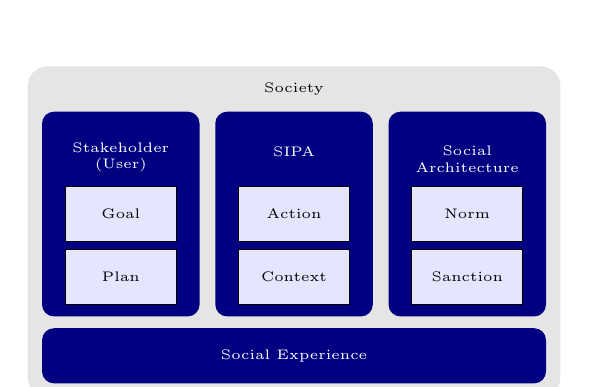
\begin{tikzpicture}[auto, node distance=2cm,>=latex',font=\tiny]
\tikzset{block/.style = {draw, rectangle, minimum height=2em, 
  minimum width=4em}}
\pgfdeclarelayer{background}
\pgfdeclarelayer{foreground}
\pgfsetlayers{background,main,foreground}

  \begin{pgfonlayer}{foreground}
    \node[block, fill=blue!10] (goal){Goal};
    \node[block, fill=blue!10, node distance=.8cm, below of=goal] 
      (plan){Plan};

    \node[block, fill=blue!10, node distance=2.2cm, right of=goal] 
      (action){Action};
    \node[block, fill=blue!10, node distance=.8cm, below of=action] 
      (context){Context};
  
    \node[block, fill=blue!10, node distance=2.2cm, right of=action] 
      (norm){Norm};
    \node[block, fill=blue!10, node distance=.8cm, below of=norm] 
      (sanction){Sanction};
  
  \end{pgfonlayer}
  
  \node[fit= (goal) (plan), inner sep=.5em, align=center, 
    minimum height = 2.6cm, minimum width = 2cm, yshift=.4cm,
    fill=blue!50!black, rounded corners=.15cm,
    label={[yshift=-.9cm, align=center, text=white]
    Stakeholder\\ (User)}](stakeholder){};

  \node[fit= (action) (context), right of=stakeholder,
    node distance=2.2cm,
    inner sep=.5em, align=center, 
    minimum height = 2.6cm, minimum width = 2cm,
    fill=blue!50!black, rounded corners=.15cm,
    label={[yshift=-.7cm, align=center, text=white]SIPA}]
    (sipa){};
  
  \node[fit= (norm) (sanction), right of=sipa,
    node distance=2.2cm,
    inner sep=.5em, align=center, 
    minimum height = 2.6cm, minimum width = 2cm,
    fill=blue!50!black, rounded corners=.15cm,
    label={[yshift=-.9cm, align=center, text=white]Social\\Architecture}]
    (socialarchitecture){};

  \node[node distance=1.8cm, below of=sipa, minimum height=.7cm,
    fill=blue!50!black, rounded corners=.15cm,
    text=white, minimum width=6.4cm] 
    (socialexperience){Social Experience};

  \begin{pgfonlayer}{background}
  \node[fit= (stakeholder) (sipa) (socialarchitecture)
    (socialexperience), rounded corners=.25cm, fill=gray!20,
    inner sep=.5em, align=center, yshift=.2cm,
    minimum height = 4.2cm, minimum width = 2cm,
    label={[yshift=-.5cm, align=center]Society}]
    (society){};
  \end{pgfonlayer}

\end{tikzpicture}
}
\caption{A conceptual model of the \frameworkB society.}
\label{fig:precious-model} \end{figure}

\begin{description}
\item[The stakeholders] are users. Each stakeholder has goals and plans.

\begin{itemize}[nosep]
  \item A \emph{goal} is a set of desirable states. A goal is
    associated with one or more stakeholder; each stakeholder may have multiple
    goals.
  \item A \emph{plan} is a set of actions that can bring about a goal.
    A plan is associated with a user and potentially helps bring about 
    one or more goals of that user.
\end{itemize}

\item[The social architecture] of a society consists of its norms
and the sanctions that ensure compliance and noncompliance of norms.

\begin{itemize}[nosep]
%   \item A \emph{norm} is directed from a subject (stakeholder) to an
%     object (stakeholder), and is constructed as a conditional
%     relationship involving an antecedent (which brings the norm in
%     force) and a consequent (which brings the norm to satisfaction or
%     violation) \citep{Singh-2013-Norms}.  
  \item A \emph{norm} is a tuple of \{subject, object, antecedent, consequent\} \citep{Singh-2013-Norms}. 
    Norms  characterize the social architecture that promotes prosocial behavior. 
  \item A \emph{sanction} is a set of actions a stakeholder may take
    for deviation of a norm by another stakeholder.  Depending on how
    agents perceive deviation, it results in \emph{sanctions} that are
    positive or negative \citep{Nardin-KER16-Classifying}.
\end{itemize}

\item[A SIPA] acts and interacts on behalf of a stakeholder and
is aware of the social architecture of the society.

\begin{itemize}[nosep]
  \item An \emph{action} is a step a SIPA takes to execute its
    stakeholder's plan, thereby bringing about the corresponding goal.
    An action may satisfy or violate a norm. SIPAs in the society can
    observe each other's actions. 
%   \mps{Define action as part of a plan earlier instead of this para} 
%   \nsa{In the model, we define plans as part of a user, and action as part of a SIPA. We could move plans to SIPA.}
  \item A \emph{context} is the circumstance under which a SIPA takes
    an action \citep{Dey-2001-Context}. Thus, a context may characterize the circumstance in
    which a norm is satisfied or violated. A SIPA may share the
    context in which it takes an action with other SIPAs.
\end{itemize}

\item[Experience] captures which or how many goals of its stakeholders a SIPA helps to bring about. %\nsa{Added}

\item[Social experience] captures which goals that relate to norms are promoted by a SIPA. 
It also relates to how a SIPA's stakeholders perceive a
norm satisfaction or violation, and the sanctions they apply. Our
objective is to promote each SIPA's actions that maximize the
social experience. %\nsa{Updated}
\end{description}

\subsection{Interaction and Learning}

%\nsa{add line-by-line explanation}

Algorithm~\ref{alg:interaction} shows how SIPAs interact and learn in
\frameworkB. Further, each SIPA, to bring about its goals, identifies
plans and an associated set of actions for each goal. If multiple plans
can achieve a goal, the SIPA selects the plan that yields the larger
social experience (based on its history), or the first viable plan. The
actions a SIPA performs as part of a plan are observed by all other
SIPAs. As SIPAs execute plans, they share the associated context with
other SIPAs.

When other SIPAs observe a SIPA's actions and receive its shared
context, they sanction it. Each SIPA stores the goals, plans, associated
context, and sanctions received in its history to facilitate future
decision making.

\begin{algorithm}[!htb]
\caption{Interaction and learning in \frameworkB.}
\label{alg:interaction}
% \small
\KwIn{$N$: norms}
\KwIn{$g$: goal}
\KwIn{$P$: plans}
\KwIn{$c$: context}
$p_{exec}$ = $\emptyset$\;
$e_{max}$ = $0$\; 
%\ForEach{$p_i \in P \vdash (G \mid c)$}{
\ForEach{$p_i \in P$ where $p_i$ satisfies $g$ under $c$}{
  $h$ = hasHistory($G$, $p$, $c$)\;
% \eIf{$h \neq \emptyset$}{
 \eIf{$h$}{
  $exp_i$ = predictExperience($p_i$, $c$, $h$)\;
  \If{$exp_i > e_{max}$}{
  $exp_{max}$ = $exp_i$\;
  $p_{exec}$ = $p_i$\;
  }
 }{
  $p_{exec}$ = $p_i$\;
 }
}
  Perform plan $p_{exec}$\;
  Share context \{$p_{exec}$, $c$\}\;
  Receive sanctions \{$s$\}\;
  Add history \{$g$, $p_{exec}$, $c$, $s$\}\;      
\end{algorithm}


        

\subsection{Example SIPA: \ringer}
\label{sec:ringer-framework}
We demonstrate \frameworkB using an example SIPA called \ringer,
whose conceptual model Figure~\ref{fig:xipho-ringer-as-is} shows 
\citep{Murukannaiah-AAMAS14-Xipho}. The \fsl{callee}, a
stakeholder of \ringer, has the goals of \fsl{being reachable by
phone}, \fsl{to work uninterrupted}, \fsl{to not disturb neighbors}
and \fsl{to preserve privacy}. The \fsl{caller}, another stakeholder,
has the goal \fsl{to reach the callee}.  The \fsl{neighbor}, also
a stakeholder, has a goal \fsl{to not be disturbed}. To provide a
rich social experience to its stakeholders, the SIPA should be aware
of its context, stakeholders' goals, associated plans, and the applicable 
norms. 

%\begin{figure}[!htb] \centering
%\includegraphics[angle=0,width={0.75\columnwidth}]{Chapter-3/fig/ringer-manager-tropos-actor-model.pdf}
%\caption{A conceptual model of the \ringer agent, expanding the
%  \fsl{callee}'s perspective \protect\citep{Murukannaiah-AAMAS14-Xipho}.\nsa{TBD: replace + add privacy}}
%\label{fig:xipho-ringer-as-is} \end{figure}

    
Following Algorithm~\ref{alg:interaction}, the \ringer starts
interacting with other agents, considering a fixed set of norms, such as
\fsl{never answer a call during a meeting} or \fsl{always answer an
urgent call from a family member}. As it acts and interacts with its
users, it learns contextually relevant norms and appropriate actions.

Algorithm~\ref{alg:decision-making} describes decision making for an
incoming phone call for a \ringer that has history. Here the
\fsl{context} includes the caller-callee relationship, call urgency
(casual or urgent), the place where the callee is, and the
neighbor-callee relationship. Possible plans include answering or
ignoring the incoming phone call. To make a choice, the \ringer predicts
the experience for the two plans from its history and chooses the action
that provides the higher social experience. Note that, to predict
experience for each action, SIPA could employ any machine learning
technique, such as linear regression, on the accumulated history. But
machine learning is not the core focus here.

%\mps{locale=environment?}

\begin{algorithm}[ht]
% \small
\caption{$a$ $\leftarrow$ selectAction($r_c$, $u$, $l$, $r_n$, $h$).}
\label{alg:decision-making}
\KwIn{$r_c$: caller-callee relationship}
\KwIn{$u$: call urgency}
\KwIn{$l$: place}
\KwIn{$r_n$: neighbor-callee relationship}
\KwIn{$h$: History}
\KwOut{$a$: action}
$exp_{answer}$ = predictExperience($h$, Answer, $r_c$, $l$, $r_n$)\;
$exp_{ignore}$ = predictExperience($h$, Ignore, $r_c$, $l$, $r_n$)\;
\eIf{$exp_{answer}>exp_{ignore}$}
{$a$ = Answer}
{$a$ = Ignore}
\end{algorithm}


As the \fsl{callee}'s \ringer chooses an action, it follows
Algorithm~\ref{alg:context-sharing} to share the context with all
\fsl{neighbors} and the \fsl{caller}. A SIPA identifies the norms that
are satisfied or violated, and provides contextual arguments in favor of
and against why it chose its action given norm satisfaction and
violation. Ideally, \ringer should selectively reveal contexts to other
stakeholders according to its goals and its human user's privacy
attitude. However, for simplicity, we have \ringer share context with
all stakeholders. The sharing of contexts can lead to additional
benefits such as increase in trust between users. We do not model those
in the current work.


\begin{algorithm}[ht]
% \small
\caption{$c$ $\leftarrow$ shareContext($N$, $a$, $r_c$, $u$, $l$, $r_n$).}
\label{alg:context-sharing}
\KwIn{$N$: norms}
\KwIn{$a$: action}
\KwIn{$r_c$: caller-callee relationship}
\KwIn{$u$: call urgency}
\KwIn{$l$: place}
\KwIn{$r_n$: neighbor-callee relationship}
\KwOut{$c$: context arguments}

\ForEach{$n_i \in N$}{
 \If{$isSatisfied(n_i, a)$}{
   Add ContextArgInFav $\leftarrow$ ($n_i$, $a$, $r_c$, $l$, $r_n$);
   }
 \If{$isViolated(n_i, a)$}{
   Add ContextArgInOpp $\leftarrow$ ($n_i$, $a$, $r_c$, $l$, $r_n$);
   }
}
\If{ContextArgInFav $\neq \emptyset$ $\lor$ ContextArgInOpp $\neq \emptyset$}{
 $c$ = \{ContextArgInFav, ContextArgInOpp\}\;
}
\end{algorithm}

When a \ringer instance receives the context shared by another \ringer
instance, the receiver reasons about context as detailed in
Algorithm~\ref{alg:reasoning-context}. Consider the \fsl{caller}'s
\ringer, for example. When \fsl{callee}'s \ringer shares the context
with the \fsl{caller}'s \ringer, the latter predicts an action according
to its history of incoming calls. If the \fsl{caller}'s predicted action
based on its history matches the \fsl{callee}'s observed action, the
\fsl{caller} positively sanctions the \fsl{callee}; otherwise the
\fsl{caller} perceives the \fsl{callee} as a deviant, and negatively
sanctions it. The \fsl{neighbor}'s \ringer sanctions the \fsl{callee}
similarly.

\begin{algorithm}[ht]
\caption{$s$ $\leftarrow$ reasonAboutContext($a$, $r_c$, $u$, $l$, $r_n$, $h$).}
\label{alg:reasoning-context}
\KwIn{$a$: action}
\KwIn{$r_c$: caller-callee relationship}
\KwIn{$u$: call urgency}
\KwIn{$l$: place}
\KwIn{$r_n$: neighbor-callee relationship}
\KwIn{$h$: History}
\KwOut{$s$: sanction}
$a_e$ = selectAction($r_c$, $u$, $l$, $r_n$, $h$)\;
\eIf{$a = a_e$}{
 $s$ = $s_p$: positive sanction\;
}
{
 $s$ = $s_n$: negative sanction\;
}
\end{algorithm}

\section{Simulation Model}
\label{sec:precious-simulation-model}

We evaluate \frameworkB via a simulation model. 
We use MASON \citep{Luke-2005-Mason} to build a simulation environment, 
henceforth the \emph{ringer environment}, inspired from real-life settings 
where the \ringer can interact.  

\subsection{The Ringer Environment}
The ringer environment contains shared places, as
Figure~\ref{fig:ringer-environment} shows. Each place is a location such
as home, party, meeting, library, and emergency room understood in
conceptual terms \citep{IC-Platys-12}. Corresponding to each place, we
define social circles such as family, friends, and colleagues. Each
agent belongs to one or more of these circles. The agents keep moving
from place to place. Network topology is random but each agent is part
of three circles: friend, family and colleague.

\begin{figure}[!htb] \centering
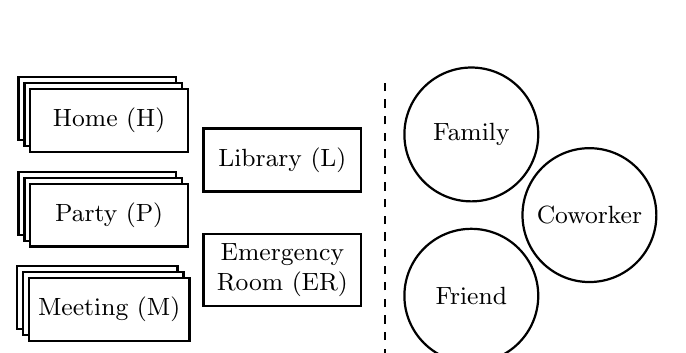
\begin{tikzpicture}[auto, node distance=2cm,>=latex',font=\small]
\tikzset{%
  cascaded/.style = {%
    general shadow = {%
      shadow scale = 1,
      shadow xshift = -1ex,
      shadow yshift = 1ex,
      draw,
      thick,
      fill = white},
    general shadow = {%
      shadow scale = 1,
      shadow xshift = -.5ex,
      shadow yshift = .5ex,
      draw,
      thick,
      fill = white},
    fill = white, 
    draw,
    thick,
    minimum width = 2cm,
    minimum height = .8cm
  }
}
  
  \node[cascaded] (home){Home (H)};
  \node[cascaded, node distance=1.2cm, below of=home] (party){Party (P)};
  \node[cascaded, node distance=1.2cm, below of=party]
    (meeting){Meeting (M)};

  \node[draw, thick, minimum width=2cm, minimum height=.8cm,
    yshift=-.5cm,
    node distance=2.2cm, right of=home] (library){Library (L)};
  \node[draw, thick, minimum width=2cm, minimum height=.8cm,
    yshift=.5cm,
    node distance=2.2cm, right of=meeting, align=center] 
    (emergencyroom){Emergency\\Room (ER)};

  \draw [dashed,thick,right of=library] (1.5,-3) -- (1.5,.5);

  \node[draw, thick, circle, minimum size=1.7cm, yshift=-.5em,
    node distance=4.6cm, right of=home] (family){Family};
  \node[draw, thick, circle, minimum size=1.7cm, yshift=.5em,
    node distance=4.6cm, right of=meeting] (friend){Friend};
  \node[draw, thick, circle, minimum size=1.7cm,
    node distance=6.1cm, right of=party] (coworker){Coworker};
\end{tikzpicture}
\caption{Places and social circles in the ringer environment.}
\label{fig:ringer-environment} \end{figure}

%\begin{figure}[!htb] \centering
%\includegraphics[angle=0,width={0.95\columnwidth}]{Chapter-3/fig/ringer-environment}
%\caption{Places and social circles in the ringer environment.}
%\label{fig:ringer-environment} \end{figure}


\paragraph*{Actions.}
The agents in the ringer environment perform the following actions depending upon their roles:
\begin{itemize}
\item A caller initiates an urgent or a casual phone call.
\item A callee answers or ignores a phone call.
\item A caller and neighbors respectively sanction a callee for answering or ignoring phone calls.
\item A callee shares context for answering or ignoring phone calls.
\item A caller and a neighbor reason about context.
\end{itemize}

\paragraph*{Norms.}
Each place and each circle has predefined norms, as defined in Table~\ref{tab:norms-place}.

%\nsa{Note that norms in Table 1 (a) and (b) could conflict. E.g., 
%A casual or urgent phone call from a family member when an agent is in 
%a meeting. We do not list down all the norms but let the agents learn 
%contextually relevant norms in case of conflict.}


\begin{table}[!htb]
\centering
% \small
\caption[Norms for answering calls.]{Norms for answering calls based on the place and the caller's social circle.}
\label{tab:norms-place}

\begin{tabular}{c}

\begin{tabular}{lc}
\toprule
\fbf{Place} & \fbf{Answer}\\\midrule
Home (H) & \cmark \\
Party (P) &\cmark\\
Meeting (M) &\xmark\\
Library (L) &\xmark\\
Emergency (ER) &\cmark\\
\bottomrule
\end{tabular}

\\
\vspace{2em}
\\

\begin{tabular}{lcc}
\toprule
\multirow{2}{*}{\fbf{Circle}}&\multicolumn{2}{c}{\fbf{Call Type}}\\\cmidrule{2-3}
&Casual&Urgent\\
\midrule
Family&\cmark&\cmark\\
Friend&\cmark&\cmark\\
Coworker&\cmark&\cmark\\
Stranger&\xmark&\cmark\\
\bottomrule
\end{tabular}


\end{tabular}


\end{table}

\paragraph*{ Payoffs.} For each phone call, based on the callee's action of answering or not answering, the 
caller, callee, and neighbors perceive a fixed payoff
as shown in Tables~\ref{tab:payoff-callee}, \ref{tab:payoff-caller} 
and \ref{tab:payoff-neighbor}. 


\begin{table}[!htb]
\centering
% \small
\caption{Payoff for the callee.}
\label{tab:payoff-callee}
\begin{tabular}{lcrr}
\toprule
\multirow{2}{4.5cm}{\fbf{Caller's Relation}} &\multirow{2}{2.5cm}{\fbf{Callee's Response}}&\multicolumn{2}{c}{\fbf{Call Type}}\\
\cmidrule{3-4}
&&Casual&Urgent\\\midrule
\multirow{2}{4.5cm}{Family, Friend, or Coworker}&\cmark&0.50&1.00\\
&\xmark&0.00&--0.50\\\midrule
\multirow{2}{4.5cm}{Stranger}&\cmark&0.00&0.50\\
&\xmark&0.25&--0.25\\
\bottomrule
\end{tabular}
\end{table}

\begin{table}[!htb]
\centering
% \small
\caption{Payoff for the caller.}
\label{tab:payoff-caller}
\begin{tabular}{crr}
\toprule
\multirow{2}{*}{\fbf{Callee's Response}} &\multicolumn{2}{c}{\fbf{Call Type}}\\
\cmidrule{2-3}
&Casual&Urgent\\\midrule
\cmark&0.50&1.00\\
\xmark&--0.50&--1.00\\\bottomrule
\end{tabular}
\end{table}

\begin{table}[!htb]
\centering
% \small
\caption{Payoff for the neighbors.}
\label{tab:payoff-neighbor}
\begin{tabular}{crrrrr}
\toprule
\multirow{2}{*}{\fbf{Callee's Response}} &\multicolumn{5}{c}{\fbf{Place}}\\
\cmidrule{2-6}
% &H&M&ER&P&L\\\midrule
% \cmark&0.67&--1.00&1.00&--0.33&--1.00\\
% \xmark&--0.33&1.00&--1.00&0.67&1.00\\\bottomrule

& H & P & M & L & ER \\\midrule
\cmark&0.67&--0.33&--1.00&--1.00&1.00\\
\xmark&--0.33&0.67&1.00&1.00&--1.00\\\bottomrule

\end{tabular}
\end{table}


\subsection{Agent Types}
\label{sec:agent-types}

\emph{Fixed agents} act according to the fixed set of norms listed in
Table~\ref{tab:norms-place}. If the norms conflict, the agents toss a
fair coin to choose between alternative actions. If Fixed agents
perceive an action as deviation, they sanction the deviant.

\emph{Sanctioning agents} learn social norms from sanctions
\citep{Andrighetto-2013-PunishVoice}. In the ringer environment, these
agents start as Fixed agents. They continue to record the call history,
and associated sanctions. Once they have gained confidence about their
history of sanctions, they base their actions on the learning based on
history. That is, as callees, when norms conflict, they select the
action that provides a higher payoff, computed according to
Tables~\ref{tab:payoff-callee}--\ref{tab:payoff-neighbor}. As callers
and neighbors, these agents sanction callees as per fixed norms listed
in Table~\ref{tab:norms-place}.

\emph{\frameworkB agents} learn social norms by sharing and reasoning
about context. In the ringer environment, \frameworkB agents start as Fixed
agents following fixed norms listed in Table~\ref{tab:norms-place}. As
callees, they share context, i.e., reveal the caller's relationship and
the call's urgency, to their neighbors, and reveal their place and their
neighbors' relationships to the caller. As neighbors or callers, they
first understand a callee's context and decide what action they would
have performed were they in the same situation, and sanction
accordingly. \frameworkB agents use payoffs as listed in
Table~\ref{tab:payoff-neighbor-reason}.

In the simulation, we employ a linear regression model over history to
predict sanctions by stakeholders, and thus social experience.

\begin{table}[!htb]
\centering
% \small
\caption[Payoffs based on reasoning about the shared context.]{Payoff for the neighbors based on reasoning about the shared context by the callee.}
\label{tab:payoff-neighbor-reason}
\begin{tabular}{ccrrrrr}
\toprule
\multirow{2}{2.5cm}{\fbf{Callee's Response}}&\multirow{2}{2.8cm}{\fbf{Neighbor's Expectation}}&\multicolumn{5}{c}{\fbf{Place}}\\
\cmidrule{3-7}
&&H&M&ER&P&L\\\midrule
\cmark&\cmark &0.67 &1 &1 &0.67&1\\
\cmark&\xmark &--0.33 &--1 &--1 &--0.33&--1\\
\xmark&\cmark &--0.33 &--1 &--1 &--0.33&--1\\
\xmark&\xmark &0.67&1&1 &0.67&1\\\bottomrule
\end{tabular}
\end{table}



\section{Experiments and Results}
\label{sec:precious-experiments}

We evaluate our research questions via three experiments in which we
simulate the agents described in
Section~\ref{sec:agent-types} on the ringer environment. We run each
simulation for $3,000$ steps and compute the following metrics.

\begin{description}
\item[Happiness] measures the proportion of agents that perceive actions
as norm compliant or respecting privacy.

\item[Experience-payoff] measures the social experience delivered by an agent. 
It is computed by aggregating payoffs for all stakeholders according to
the payoff Tables~\ref{tab:payoff-callee}, \ref{tab:payoff-caller},
\ref{tab:payoff-neighbor}, and \ref{tab:payoff-neighbor-reason}.

\end{description}

To answer \fsl{RQ 1}, we consider the following hypotheses:
\begin{description}
\item[H1$_{alt}$] \frameworkB agents yield \fsl{happiness} greater than that yielded by Fixed agents.
\item[H1$_{null}$] \frameworkB agents yield no significant gain in \fsl{happiness} over Fixed agents.
\item[H2$_{alt}$] \frameworkB agents yield \fsl{happiness} greater than that yielded by Sanctioning agents.
\item[H2$_{null}$]  \frameworkB agents yield no significant gain in \fsl{happiness} over Sanctioning agents.
\end{description}

To answer \fsl{RQ 2}, we consider the following hypotheses:
\begin{description}
\item[H3$_{alt}$] \frameworkB agents yield \fsl{social experience} greater than that yielded by Fixed agents.
\item[H3$_{null}$] \frameworkB agents yield no significant gain in \fsl{social experience} over Fixed agents.
\item[H4$_{alt}$] \frameworkB agents yield \fsl{social experience} greater than that yielded by Sanctioning agents.
\item[H4$_{null}$]  \frameworkB agents yield no significant gain in \fsl{social experience} over Sanctioning agents.
\end{description}

To test the significance of the hypotheses, we apply the common two-tailed paired $t$-test. 

\subsection{Pragmatic Agents and Varying Network Size}
\label{sec:experiment1}

We simulate agents described in Section~\ref{sec:agent-types} on four
types of network, specifically, large and small networks with dense or
sparse connectivity as Table~\ref{tab:network-types} describes. The
agents in this experiment are pragmatic, and try to achieve a high average
experience-payoff for all callees, callers, and neighbors. We now
describe our results.

\begin{table}[!htb]
\centering
\caption{Characteristics of network types studied.}
\label{tab:network-types}
\begin{tabular}{crrrr}
\toprule
\multirow{2}{*}{\fbf{Network Type}} & \multirow{2}{*}{\fbf{Agents}} & \multicolumn{3}{c}{\fbf{Circles}}\\
\cmidrule{3-5}
&&Home&Meeting&Party\\
\midrule
Large-Dense&1,000&20&20&20\\
Large-Sparse&1,000&100&100&100\\
Small-Dense&250&5&5&5\\
Small-Sparse&250&25&25&25\\
\bottomrule
\end{tabular}
\end{table}



\begin{description} \item[Fixed agents.] behave
according to the fixed norms, their behaviors do not change over time.
As expected, we observe no significant change in social experience
throughout the simulation. The average social experience was found to be
between $0.53$ and $0.56$, and the happiness to be about $52$\% for the
four network types.

\item[Sanctioning agents.] Sanctioning agents first learn and then act as they
have learned. As expected, at around step $1,000$ we see a rise in
social experience offered by Sanctioning compared to Fixed agents. The rise
is gradual as the agents start to learn. For the first $200$ steps, the
average social experience is the same as Fixed agents. It later
stabilizes between $1.11$ and $1.21$ for all four networks. The happiness
values were between $61.2$ and $63.7$\%.

\item[\frameworkB agents.] \frameworkB agents first learn, and then act according
to the learning. At around step $1,000$, as agents acquire confidence,
we see a significant increase in social experience offered by \frameworkB
agents. It stabilizes between $2.14$ and $2.19$ for the different networks.
Happiness was found be significantly higher between $82.0$ and $83.2$\%.
For the first $200$ steps, \frameworkB agents yield the same average social
experience as Fixed and Sanctioning agents. \end{description}

Happiness and experience payoffs offered by \frameworkB agents are 
significantly greater than those offered by Fixed and Sanctioning agents;
thus the four null hypotheses: H1$_{null}$, H2$_{null}$, H3$_{null}$,
and H4$_{null}$, are rejected. Figure~\ref{fig:experiment1-results} show
the experience payoff plots indicating the results are consistent across
the four network types. Table~\ref{tab:experiment1-results} summarizes
the findings of the experiment with pragmatic agents.

\begin{figure}[!htb]
    \centering
    
\begin{tabular}{cc}

    \begin{tikzpicture}
    \begin{axis}[
        title={Large-Dense Network},
        height=7cm,
        width=7cm,
        xlabel={Step},
%         ylabel={Average Payoff Within a Window \%},
        ylabel={Experience payoff},
        xmin=0, xmax=3001,
        ymin=0, ymax=3,
%        xtick={1,2,3,4,5,6,7,8,9,10},
%         ytick={25,50,75,100},
         legend pos=north west,
        legend style={font=\small},
        ymajorgrids=true,
        grid style=dashed,
        ]

        \addplot table [x=Step, y=Avg Payoff in Window, col sep=comma, mark=none] {Chapter-3/data/LD_Sim3.csv}; 
        \addplot table [x=Step, y=Avg Payoff in Window, col sep=comma, mark=none] {Chapter-3/data/LD_Sim2.csv};
        \addplot table [x=Step, y=Avg Payoff in Window, col sep=comma, mark=none] {Chapter-3/data/LD_Sim1.csv};

        \addplot +[mark=none,dashed] coordinates {(1000, -1) (1000, 3)};
         \legend{\frameworkB,Sanctioning,Fixed}
    \end{axis}
    \end{tikzpicture}
%     \caption{Average payoff per call for a window size of 200 steps for a large-dense network}
%     \label{fig:experiment-1-ld-results}
% \end{figure}


&

% \begin{figure}[!htb]
% \centering

    \begin{tikzpicture}
    \begin{axis}[
        title={Large-Sparse Network},
        height=7cm,
        width=7cm,
        xlabel={Step},
%         ylabel={Average Payoff Within a Window \%},
%         ylabel={Average payoff},
        xmin=0, xmax=3001,
        ymin=0, ymax=3,
%        xtick={1,2,3,4,5,6,7,8,9,10},
%         ytick={25,50,75,100},
        legend pos=north west,
        legend style={font=\tiny},
        ymajorgrids=true,
        grid style=dashed,
        ]
         \addplot table [x=Step, y=Avg Payoff in Window, col sep=comma, mark=none] {Chapter-3/data/LS_Sim3.csv};
         \addplot table [x=Step, y=Avg Payoff in Window, col sep=comma, mark=none] {Chapter-3/data/LS_Sim2.csv};
         \addplot table [x=Step, y=Avg Payoff in Window, col sep=comma, mark=none] {Chapter-3/data/LS_Sim1.csv};
         \addplot +[mark=none,dashed] coordinates {(1000, -1) (1000, 3)};
%         \legend{P,S,F}
    \end{axis}
    \end{tikzpicture}
%     \caption{Average payoff per call for a window size of 200 steps for a large-sparse network}
%     \label{fig:experiment-1-ls-results}
% \end{figure}


\\

% \begin{figure}[!htb]
%     \centering

\begin{tikzpicture}
    \begin{axis}[
        title={Small-Dense Network},
        height=7cm,
        width=7cm,
        xlabel={Step},
%         ylabel={Average Payoff Within a Window \%},
        ylabel={Experience payoff},
        xmin=0, xmax=3001,
        ymin=0, ymax=3,
%        xtick={1,2,3,4,5,6,7,8,9,10},
%         ytick={25,50,75,100},
        legend pos=north west,
        legend style={font=\tiny},
        ymajorgrids=true,
        grid style=dashed,
        ]
         \addplot table [x=Step, y=Avg Payoff in Window, col sep=comma, mark=none] {Chapter-3/data/SD_Sim3.csv};
         \addplot table [x=Step, y=Avg Payoff in Window, col sep=comma, mark=none] {Chapter-3/data/SD_Sim2.csv};
         \addplot table [x=Step, y=Avg Payoff in Window, col sep=comma, mark=none] {Chapter-3/data/SD_Sim1.csv};
         \addplot +[mark=none,dashed] coordinates {(1000, -1) (1000, 3)};
%         \legend{P,S,F}
    \end{axis}
    \end{tikzpicture}
%     \caption{Average payoff per call for a window size of 200 steps for a large-dense network}
%     \label{fig:experiment-1-sd-results}
% \end{figure}


&
% \begin{figure}[!htb]
%     \centering
    \begin{tikzpicture}
    \begin{axis}[
        title={Small-Sparse Network},
        height=7cm,
        width=7cm,
        xlabel={Step},
%         ylabel={Average Payoff Within a Window \%},
%         ylabel={Average payoff},
        xmin=0, xmax=3001,
        ymin=0, ymax=3,
%        xtick={1,2,3,4,5,6,7,8,9,10},
%         ytick={25,50,75,100},
        legend pos=south east,
        legend style={font=\tiny},
        ymajorgrids=true,
        grid style=dashed,
        ]
        \addplot table [x=Step, y=Avg Payoff in Window, col sep=comma, mark=none] {Chapter-3/data/SS_Sim3.csv};
        \addplot table [x=Step, y=Avg Payoff in Window, col sep=comma, mark=none] {Chapter-3/data/SS_Sim2.csv};
        \addplot table [x=Step, y=Avg Payoff in Window, col sep=comma, mark=none] {Chapter-3/data/SS_Sim1.csv};
         \addplot +[mark=none,dashed] coordinates {(1000, -1) (1000, 3)};
%          \legend{P,S,F}
    \end{axis}
    \end{tikzpicture}

\\
\end{tabular}

\caption[Experience payoff plots for different networks.]{Experience payoff per phone call for a window size of $200$
steps on different network sizes and densities.}
    \label{fig:experiment1-results}
\end{figure}

\begin{table*}[!htb]
% \smaller
\caption{Empirical results on the effectiveness of \frameworkB agents.}
\label{tab:experiment1-results}
\centering

\begin{tabular}{c}

Large-Dense 
\\

\begin{tabular}{lrrr}
\toprule
Agent Type & Experience$^\#$ & Happiness$^{\#\#}$ & $p^{\#\#\#}$\\
\midrule
Fixed & $0.56$ &$52.7\%$ & $< 0.01$\\
Sanctioning & $1.21$ &$63.5\%$ & $< 0.01$\\
\frameworkB & $2.19$&$83.2\%$ & -- \\
\bottomrule
\end{tabular}
\vspace{1em}
\\
Large-Sparse
\\
\begin{tabular}{lrrr}
\toprule
Agent Type & Experience$^\#$ & Happiness$^{\#\#}$ & $p^{\#\#\#}$\\
\midrule
Fixed &$0.55$  &$52.5\%$ & $< 0.01$\\
Sanctioning &$1.21$  &$63.5\%$ & $< 0.01$\\
\frameworkB &$2.19$ &$83.2\%$ & --\\
\bottomrule
\end{tabular}
\vspace{1em}
\\
Small-Dense 
\\
\begin{tabular}{lrrr}
\toprule
Agent Type & Experience$^\#$ & Happiness$^{\#\#}$ & $p^{\#\#\#}$\\
\midrule
Fixed &$0.53$  &$52.1\%$ & $< 0.01$\\
Sanctioning &$1.11$  &$61.2\%$ & $< 0.01$\\
\frameworkB &$2.14$ &$82.0\%$ & --\\
\bottomrule
\end{tabular}
\vspace{1em}
\\
Small-Sparse
\\
\begin{tabular}{lrrr}
\toprule
Agent Type & Experience$^\#$ & Happiness$^{\#\#}$ & $p^{\#\#\#}$\\
\midrule
Fixed &$0.54$  &$52.5\%$ & $< 0.01$\\
Sanctioning &$1.22$  &$63.7\%$ & $< 0.01$\\
\frameworkB &$2.14$ &$82.1\%$ & --\\
\bottomrule
\end{tabular}
\vspace{1em}
\\

\multicolumn{1}{l}{$^\#$ Stabilized value of social experience;}\\
\multicolumn{1}{l}{$^{\#\#}$ Stabilized value of happiness;}\\
\multicolumn{1}{l}{$^{\#\#\#}$ Two-tailed paired $t$-test}

\end{tabular}

\end{table*}

\subsection{Experiment with Considerate Agents} 
We experiment with considerate agents who consider payoffs only for
their neighbors when deciding the actions to perform when norms
conflict. These agents continue to sanction based on their history.

\paragraph{Results.} Figure~\ref{fig:experiment2-considerate-selfish}
shows the experience payoffs for considerate Sanctioning and \frameworkB
agents in a Small-Dense network. The average experience payoff drops for
Sanctioning and \frameworkB agents after they have gained enough
confidence. We attribute this decline to the fact that these agents
value the neighbors' experience payoff more than their own, and thus
start to ignore calls that they should have answered. \frameworkB agents
offer higher experience payoff than Sanctioning agents because the
stakeholders give smaller negative sanctions when they reason about
context. The results for the other three network types are similar.

\subsection{Experiment with Selfish Agents} 
Selfish agents consider only their payoffs when performing actions.
Selfish agents may not always sanction others. They sanction a deviant
based on their history.

\paragraph{Results.} Figure~\ref{fig:experiment2-considerate-selfish}
shows the experience payoff plot for selfish Fixed and \frameworkB agents
in a Small-Dense network. The plots are similar to those in the
experiment with pragmatic agents, but with slightly lower stabilized
values. Here, agents tend to answer all calls, which benefits both
caller and callee most of the time. We observe similar results for the
other three networks.

\begin{figure}[!htb]
\centering
\begin{tabular}{cc}
    \begin{tikzpicture}
    \begin{axis}[
        title={Considerate Agents},
        height=7cm,
        width=7cm,
        xlabel={Step},
%         ylabel={Average Payoff Within a Window \%},
        ylabel={Experience payoff},
        xmin=0, xmax=3001,
        ymin=-1, ymax=3,
%        xtick={1,2,3,4,5,6,7,8,9,10},
%         ytick={25,50,75,100},
        legend pos=north west,
        legend style={font=\small},
        ymajorgrids=true,
        grid style=dashed,
        ]

         \addplot table [x=Step, y=Avg Payoff in Window, col sep=comma, mark=none] {Chapter-3/data/SS_Considerate_Sim3.csv};
          \addplot table [x=Step, y=Avg Payoff in Window, col sep=comma, mark=none] {Chapter-3/data/SS_Considerate_Sim2.csv};
         \addplot +[mark=none,dashed] coordinates {(1000, -1) (1000, 3)};
        \legend{\frameworkB,Sanctioning}
    \end{axis}
    \end{tikzpicture}
% \caption{Experience with considerate agents}
% \label{fig:considerate}
% \end{subfigure}
&
% \begin{subfigure}[t]{0.45\columnwidth}
%      \centering
    \begin{tikzpicture}
    \begin{axis}[
        title={Selfish Agents},
        height=7cm,
        width=7cm,
        xlabel={Step},
%         ylabel={Average Payoff Within a Window \%},
%         ylabel={Average experience},
        xmin=0, xmax=3001,
        ymin=-1, ymax=3,
%        xtick={1,2,3,4,5,6,7,8,9,10},
%         ytick={25,50,75,100},
        legend pos=north west,
        legend style={font=\small},
        ymajorgrids=true,
        grid style=dashed,
        ]

          \addplot table [x=Step, y=Avg Payoff in Window, col sep=comma, mark=none] {Chapter-3/data/SS_Selfish_Sim3.csv};
          \addplot table [x=Step, y=Avg Payoff in Window, col sep=comma, mark=none] {Chapter-3/data/SS_Selfish_Sim2.csv};
         \addplot +[mark=none,dashed] coordinates {(1000, -1) (1000, 3)};
         \legend{\frameworkB,Sanctioning}
    \end{axis}
    \end{tikzpicture}
\end{tabular}
\caption[Experience payoff plots for considerate and selfish agents.]{Experience payoffs (averaged over a window size of 200 steps)
yielded by considerate and selfish agents in a Small-Dense network.}
\label{fig:experiment2-considerate-selfish}
% \end{subfigure}
\end{figure}

\section{Conclusion and Future Directions}
\label{sec:precious-discussion}

\frameworkB is a framework in which SIPAs learn contextually relevant
social norms by offering and reasoning shared contexts. Via a series of
simulation experiments, we find that \frameworkB agents accurately learn
contextually norms compared to agents relying on fixed norms or learning
norms via sanctions. In the experiments, we also compute social metrics
and find that \frameworkB agents deliver significantly higher (1)
happiness, thereby are privacy respecting; and (2) experience payoff than
other agents. These findings are stable under changes to network size
and characteristics of agents.

Incorporating affect in relation to norms
\citep{Ferreira-AAAI13-GroupRelations} is an interesting future
direction. Another direction is to crowdsource data about real users'
information sharing preferences and attitudes, and build machine
learning techniques in a SIPA for recommending policies to its users.

%------------------------------%
\chapter{Enriching Social Experience with Values}
\label{chap:valar}
%------------------------------%

This chapter present preliminaries for \frameworkC and \frameworkD, our
envisioned frameworks that would help SIPAs to reason about values.

\section{Introduction}
\label{sec:valar-intro}

Smart devices including phones and wearables are now essential part of
our everyday activities. Social applications such as Facebook, Twitter,
and Google Maps running on these devices help people to be aware of each
other in real-time, to stay in touch with them. While there are benefits
of using these applications, some issues exists. For instance, consider
a location sharing application installed on a child's device via which
parents on their device could track the child's location ensuring his or
her safety. However, this obvious benefit could pose a serious security
threat if a parent's device is lost or stolen. We envision SIPAs that
are aware of, and have ability to reason about \fsl{values} to act in
ways that promotes social experience in such cases.

\paragraph*{Values}
Oxford Dictionary defines \fsl{value} (\emph{v.} with object) as
considering (someone or something) to be important or beneficial.
Rokeach based his survey proposed two sets of values---\fsl{terminal}
values and \fsl{instrumental} values \citep{rokeach1973nature}. Terminal
values refer to defined-end states of existence, and instrumental values
refer to modes of behavior or means to achieve the terminal values. We
recognize an ability to understand terminal values such as security,
freedom, happiness, and recognition, an important aspect in SIPAs to
deliver a social experience. \cite{Dechesne-AIL13-Norms+Values} define
values as ideals worth pursuing and suggest that these ideals could
conflict as they may not be preferred equally by each individual (or
each SIPA stakeholder, in our work).

\paragraph*{Values and Norms}
Few works have tried to relate values with norms.
\citet{DaSilvaFigueiredo-COIN13} propose an algorithm to identify
conflicts between norms based on values. A conflict could occur when (1)
a consequent action of a commitment norm demotes a value, or (2) a
consequent action of a prohibition norm promotes a value important to a
SIPA stakeholder. \citet{Dechesne-AIL13-Norms+Values} develop a 
model of norms and culture, represented by values, to study compliance of norms.  
They concur that values play an important role in deciding whether or 
not a norm should be introduced. \citet{kayal13coin} present a model 
of norms, context, and values with value as the central element. Such 
a model could be employed to govern a SIPA by identifying value 
preferences of SIPA's stakeholders. 

\section{SIPA and Values}

In this section we present an example SIPA.

\subsection*{\navigationapp: An Example SIPA}

Consider \navigationapp, a crowdsourced navigation app as a SIPA that
assists visually impaired in orienting themselves in cities.
\navigationapp relies on its users to contribute routes including
availability of sidewalks, crossings, and other details that could be
useful to blind people.

\navigationapp has two main components---NaviSocial and NaviAssist. 
\begin{description}
\item[NaviSocial.] Using NaviSocial, \navigationapp users can 1) share
their favorite routes, shortcuts, or secret routes with public or with
friends privately, 2) rate routes as safe or not, 3) rate routes as
adventurous or not, 4) mark potholes and other useful details, and 5)
request route recommendations.

\item[NaviAssist.] Through NaviAssist, \navigationapp users maintain a
trust-circle which includes people whom the user trusts and the app
should contact in case of an emergency. If a \navigationapp user is
disoriented, NaviAssist contacts people in disoriented user's
trust-circle to assist the user, and shares user's context (including
the place where the user is, the activity he or she is involved in, and
the people he or she is with) with the people in his or her
trust-circle.

\navigationapp users can either choose to share their contexts at all
times with their trust-circles, or only when they are disoriented.
Further, users can either choose to share abstract context (e.g., place
and relationship with neighbor), or detailed context (e.g, exact
geolocation and details of the neighbors).
\end{description}

\begin{example}
Pedro is a visually impaired masseur. His work consist of frequent
traveling around the city to visit his clients (some of which are
regular, some of which are new). Pedro already knows how to navigate
some parts of the city on his own. However, he has many clients, some
new, and he often needs to use a special navigation system to help him
move around unfamiliar areas of the city.
\end{example}

Recently, Pedro acquired \navigationapp and is excited to use it. He
adds his friends Antonio and Bruno (who are not blind) in his
trust-circles. Pedro now expects to be more independent, be able to
travel more freely and get more work done.

We note the following norms in this example. 

\begin{itemize}
\item As a \navigationapp user, Pedro is committed to share routes and
other information about the shared routes that could be useful to other
users.

$\C_{sharePublic}$: $\C$(Pedro, \navigationapp, $\top$, shareRouteInfo)

\item Pedro is further committed to share his context with Antonio and
Bruno, his friends in his trust-circle, if he is disoriented.

$\C_{sharelocPA}$: $\C$(Pedro, Antonio, disoriented, shareContext
$\land$ requestAssistance)

$\C_{sharelocPB}$: $\C$(Pedro, Bruno, disoriented, shareContext $\land$
requestAssistance)

\item Antonio and Bruno, as friends in Pedro's trust-circle,
are committed to Pedro to assist Pedro when he is disoriented and
reaches out for assistance.

% $\C_{assistanceAP}$: $\C$(Antonio, Pedro, requestAssistance, assist)
 $\C_{assistanceAP}$: $\C$(Antonio, Pedro, sat($\C_{sharelocPA}$), assist)

% $\C_{assistanceBP}$: $\C$(Bruno, Pedro, requestAssistance, assist)
$\C_{assistanceBP}$: $\C$(Bruno, Pedro, sat($\C_{sharelocPB}$), assist)

\end{itemize}

\paragraph*{Values and dominance.}

Consider a scenario where Pedro is disoriented and requests assistance.
\navigationapp contacts Antonio and Bruno with Pedro's context. In this
case, instances of both $\C_{assistanceAP}$ and $\C_{assistanceBP}$ are
detached.

\begin{itemize}

\item sat($C_{assistanceAP}$) $\lor$ sat($C_{assistanceBP}$) $\bup$ safety
\item sat($C_{assistanceAP}$) $\land$ sat($C_{assistanceBP}$) $\bdown$ resource 
%\nsa{Here, I am thinking of resource in terms of Antonio and Bruno's time}

\end{itemize}

%\nsa{To determine dominance, maintain a (partially) ordered set of values?}

Here, it is not necessary for both Antonio and Bruno to reach Pedro.
Whosoever is available and is near Pedro could assist him. If Antonio
is nearer and could reach Pedro faster, $\C_{assistanceAP}$ dominates
$\C_{assistanceBP}$ as it promotes safety and better utilization of
available resources.

\begin{example}
Rodrigo, Pedro's roommate, is also visually impaired. Pedro introduced
Rodrigo to \navigationapp and now Rodrigo uses it on a day-to-day
basis. Rodrigo has his elder brother, Carlos, in his trust-circle of
\navigationapp.
\end{example}

\begin{itemize}

\item Rodrigo shares his context with Carlos at all times and requests
help only when disoriented.

$\C_{sharelocRC}$: 
$\C$(Rodrigo, Carlos, $\top$, shareContext)

$\C_{reqAssistRC}$: 
$\C$(Rodrigo, Carlos, disoriented, shareContext $\land$ requestAssistance)

\item Carlos is committed to Rodrigo to assisting Rodrigo when he is disoriented.

% $\C_{assistanceCR}$: $\C$(Carlos, Rodrigo, requestAssistance, assist)
$\C_{assistanceCR}$: $\C$(Carlos, Rodrigo, sat($\C_{reqAssistRC}$), assist)

%\item As friends, Pedro and Rodrigo are committed to each other to share
%each other's \mps{doesn't make sense} secret routes. \nsa{Is it OK to
%say there are two separate commitments? Pedro is committed to Rodrigo to
%share route he knows? And Rodrigo is committed to share secrets he
%knows? Or they mutually commit to each other on sharing secrets?}
\item Pedro and Rodgrigo mutually commit to each other on sharing secret routes. 

$\C_{sharePrivatePR}$: $\C$(Pedro, Rodrigo, $\top$, shareSecretRoutes)

$\C_{sharePrivateRP}$: $\C$(Rodrigo, Pedro, $\top$, shareSecretRoutes)

\item Also, Pedro and Rodrigo are committed to each other to not reveal shared secrets to other people. 

% $\C_{notdisclosePrivatePR}$: $\C$(Pedro, Rodrigo, $\top$, $\neg$ discloseSharedRoutes)
$\C_{notdisclosePrivatePR}$: $\C$(Pedro, Rodrigo, sat($\C_{sharePrivateRP}$), $\neg$ discloseSharedRoutes)

% $\C_{notdisclosePrivateRP}$: $\C$(Rodrigo, Pedro, $\top$, $\neg$ discloseSharedRoutes)
$\C_{notdisclosePrivateRP}$: $\C$(Rodrigo, Pedro, sat($\C_{sharePrivatePR}$), $\neg$ discloseSharedRoutes)
\end{itemize}

\paragraph*{Values and dominance}

Consider a scenario where Pedro and Rodrigo go out together to explore
the city. While Pedro's \navigationapp shares his context with Antonio
and Bruno only in emergency, Rodrigo's \navigationapp shares his context
with Carlos at all times. If Carlos has a knowledge that Pedro and Rodrigo
always hangout together, following values are promoted and demoted.

\begin{itemize}
\item sat($\C_{shareLocRC}$) $\bup$ safety $\land$ prefRodrigo

\item sat($\C_{shareLocRC}$) $\bdown$ privacyPedro

\item vio($\C_{shareLocRC}$) $\bdown$ prefRodrigo
\end{itemize}

If Rodrigo's \navigationapp shares with Carlos only an abstract
context, it could respect Pedro's privacy, and yet promote safety and
Rodrigo's preference of sharing context at all times.

\begin{itemize}
\item shareAbstractContext $\bup$ safety $\land$ prefRodrigo $\land$ privacyPedro
\end{itemize}

%\nsa{There could be two commitments: $\C_{shareDetailedContext}$ and $C_{shareAbstractContext}$, and users can have preference of one over the other.  However, in certain cases, like the one above, a preferred commitment could be dominated by other commitment to respect privacy (or other values).}
%
%\nsa{Should norms promote (and demote) values? Or it would be antecedent or consequent promoting (and demoting) values?}

\section{Research Plan}

\citet{Dechesne-AIL13-Norms+Values}
model the relationship between values and compliance of norms. While they
suggest that values underlying the introduction of norms can serve as a
criteria to decide if one outcome is better than the other, their
results are based on simulation experiments. There is need to validate
these results against real data.

The \navigationapp example illustrate some of the opportunities for the
SIPAs to reason about values. Each action a \navigationapp SIPA performs,
promotes or demotes certain values. If a \navigationapp SIPA could
understand its stakeholders' preferences and reason about the values
promoted or demoted, it could learn contextually relevant norm and
perform actions that provide pleasant social experience to its
stakeholders. In this regard, we consider the following research questions: 

\begin{description}
\item[RQ 1.] How can we enable a SIPA to reason about values each of
their actions could promote or demote?
\item[RQ 2.] How can we build a decision support system to recommend
SIPAs actions to perform, and not to perform?
%\item[RQ 2.] Does an ability to reason about values each of their actions
%promote or demote help SIPAs learn contextually relevant norms, and
%hence provide a pleasing social experience to its stakeholders?
\end{description}

To address the research question of enabling a SIPA to reason about
values, we propose \frameworkC, a value-based framework. To develop
\frameworkC, we will conduct a crowdsourced experiment to learn different
contextual factors and associated values, and preferences and tradeoffs
between them.

To address the research question of building a decision support system,
we propose \frameworkD that will use the data collected via the
crowdsourced experiment.

%\nsa{\citet{Dechesne-AIL13-Norms+Values} results are based on a simulation. 
%Real data needs to be collected.}

%%------------------------------%
%\chapter*{Acknowledgments}
%\label{chap:ack}
%%------------------------------%
%
%This work has benefited from collaborations with several people.
%Chapters~\ref{chap:arnor} and \ref{chap:precious} are based on joint
%works with Pradeep K. Murukannaiah and Hui Guo.
%Chapter~\ref{chap:valar} is based on interactions with Pietro Passoti
%and M. Birna van Riemsdijk.
%
%I have also benefited from several other collaborators. Although the
%specific works I completed with them are not included in the
%dissertation, their knowledge and insights have undoubtedly influenced
%my thinking. These include the works on (1) sanction typology
%\citep{Nardin-KER16-Classifying} with Luis Gustavo Nardin, Tina
%Balke-Visser, Anup K. Kalia, and Jaime S. Sichman; (2) argumentation and
%secure service policies \citep{Ajmeri-Computer17-Aragorn} with Chung-Wei
%Hang and Simon D. Parsons; (3) sanctions and cybersecurity
%\citep{Du-HotSoS15,Du-Acyse15} with Honging Du, Bennett Narron, Shams
%Al-Amin, Emily Berglund, and Jon Doyle; (4) analytic workflow
%\citep{Yuan-RCIS15} with Guangchao Yuan, Chris Allred, Pankaj R. Telang,
%and Mark Wilson (5) norms and sociotechnical systems
%\citep{Kafali-IS16-Revani,Kafali-AAAI17-Kont} with {\"O}zg{\"u}r
%Kafal{\i}; (6) reasoning about normative conflicts
%\citep{Ajmeri-IJCAI16-Coco,Jiang-HotSoS16} with Jiaming Jiang, Rada
%Chirkova, and Jon Doyle; and (7) analysis of privacy news
%\citep{Sheshadri-PST17-News} with Karthik Sheshadri and Jessica
%Staddon.
%
%I also thank the US Department of Defense for support through the
%Science of Security Lablet at NC State University.

\bibliographystyle{plainnat}
\bibliography{Nirav,Munindar,Hui}

%%---------------------------------------------------------------------------%%
%Appendices
%\ensureoddstart
%\restoregeometry
\appendix
%\newgeometry{margin=1in,lmargin=1.25in,footskip=\chapterfootskip, includehead, includefoot}

\include{Appendix-A/Appendix-A}

%\restoregeometry

%%---------------------------------------------------------------------------%%
%\ensureoddstart
\backmatter

\end{document}